\documentclass[11pt,letterpaper]{article}
\input{headings}
\newcommand \recipeName {Whole-Orange Cake}
\newcommand \fileName {OrangeCake}
\chead{\recipeName}

\begin{document}
\input{title}

This is another dairy-free cake. It came to me from my Mom in Brazil. The original recipe processes a whole orange, with the rind and everything and uses two cups of sugar. Most likely to counter the bitterness of the white rind. I found that by doing just a bit of extra work by first zesting the orange and then removing the white pit, one can reduce the amount of sugar. 

The batter is quite liquid, thus I bake in a tubular pan with removable centre, but I put the baking pan into a baking sheet to avoid spills in the oven.

In 2017 I decided to research Greek cuisine and I discover a recipe for an old Greek semolina-orange cake that also used two whole orange, but it cooked the oranges first. I do wonder if this Brazilian recipe is a tropical version of the old Greek one.

\begin{description}

\item[Ingredients:]\ \\
	\begin{itemize}
	\item 1 whole orange
	\item 1 1/2 cup of sugar (10 1/2 oz)
	\item 1/2 teaspoon of salt
	\item 4 eggs
	\item 1 cup of flavourless cooking oil (7 1/2 oz)
	\item 2 tablespoons of baking powder
	\item 2 1/2 cups of all-purpose flour (12 1/2 oz)
	\item 1 cup of sweetened orange juice
	\end{itemize}

\item[Procedure:]\ \\
	\begin{enumerate}
	\item {\bf Preheat the oven and prep the fan}
		\begin{itemize}
		\item Preheat the oven on to 350 F.
		\item Put a clean baking sheet into the oven (you may cover it with aluminum foil to avoid spills into the baking sheet).
		\item Spray a tubular pan with removable centre.
		\end{itemize}
	\item {\bf Prep the orange}
		\begin{itemize}
		\item Put the sugar in the bowl of a food processor.
		\item Zest the whole orange and add the orange zest to the sugar.
		\item Process for about 30 seconds.
		\item Remove the white rind from the orange and discard the rind.
		\end{itemize}
	\item {\bf Finish the batter}
		\begin{itemize}
		\item Add the salt to the sugar-zest mixture.
		\item Add the peeled orange and process until it forms a liquid paste.
		\item Add the eggs to the sugar-orange-zest mixture.
		\item Process for a minute.
		\item Them slowly pour the oil through the feeding tube of the food processor with the processor running.
		\item Using a rubber spatula, transfer the content of the food processor to a large bowl.
		\item Using a large strained, sift the flour and the baking powder into the wet mixture and incorporate. Best is to do it in three batches to avoid lumps.  
		\end{itemize}
	\item {\bf Bake}
		\begin{itemize}
		\item Remove the hot baking sheet from the oven, put the prepared tubular pan on the centre.
		\item Put the batter into the prepared pan. and transfer, with the baking sheet, to the oven.
		\item Bake for about 45 minutes or until a toothpick inserted in the centre comes out very clean. 
		\item Remove from oven, put on top of a baking sheet and pour the orange juice on top of the hot cake.
		\item Let it stand for 5 minutes.
		\item Run a clean sharp and narrow knife around the edge of the tube pan and lift the center to remove the outside of the tube pan.
		\item Put the cake, with the center of the tubular pan still on, into a rack to cool.
		\item Let it cool for 30 minutes before removing the center of the pan.
		\end{itemize}
	\end{enumerate}
\end{description}

\begin{table}
\begin{tabular}{cccc}
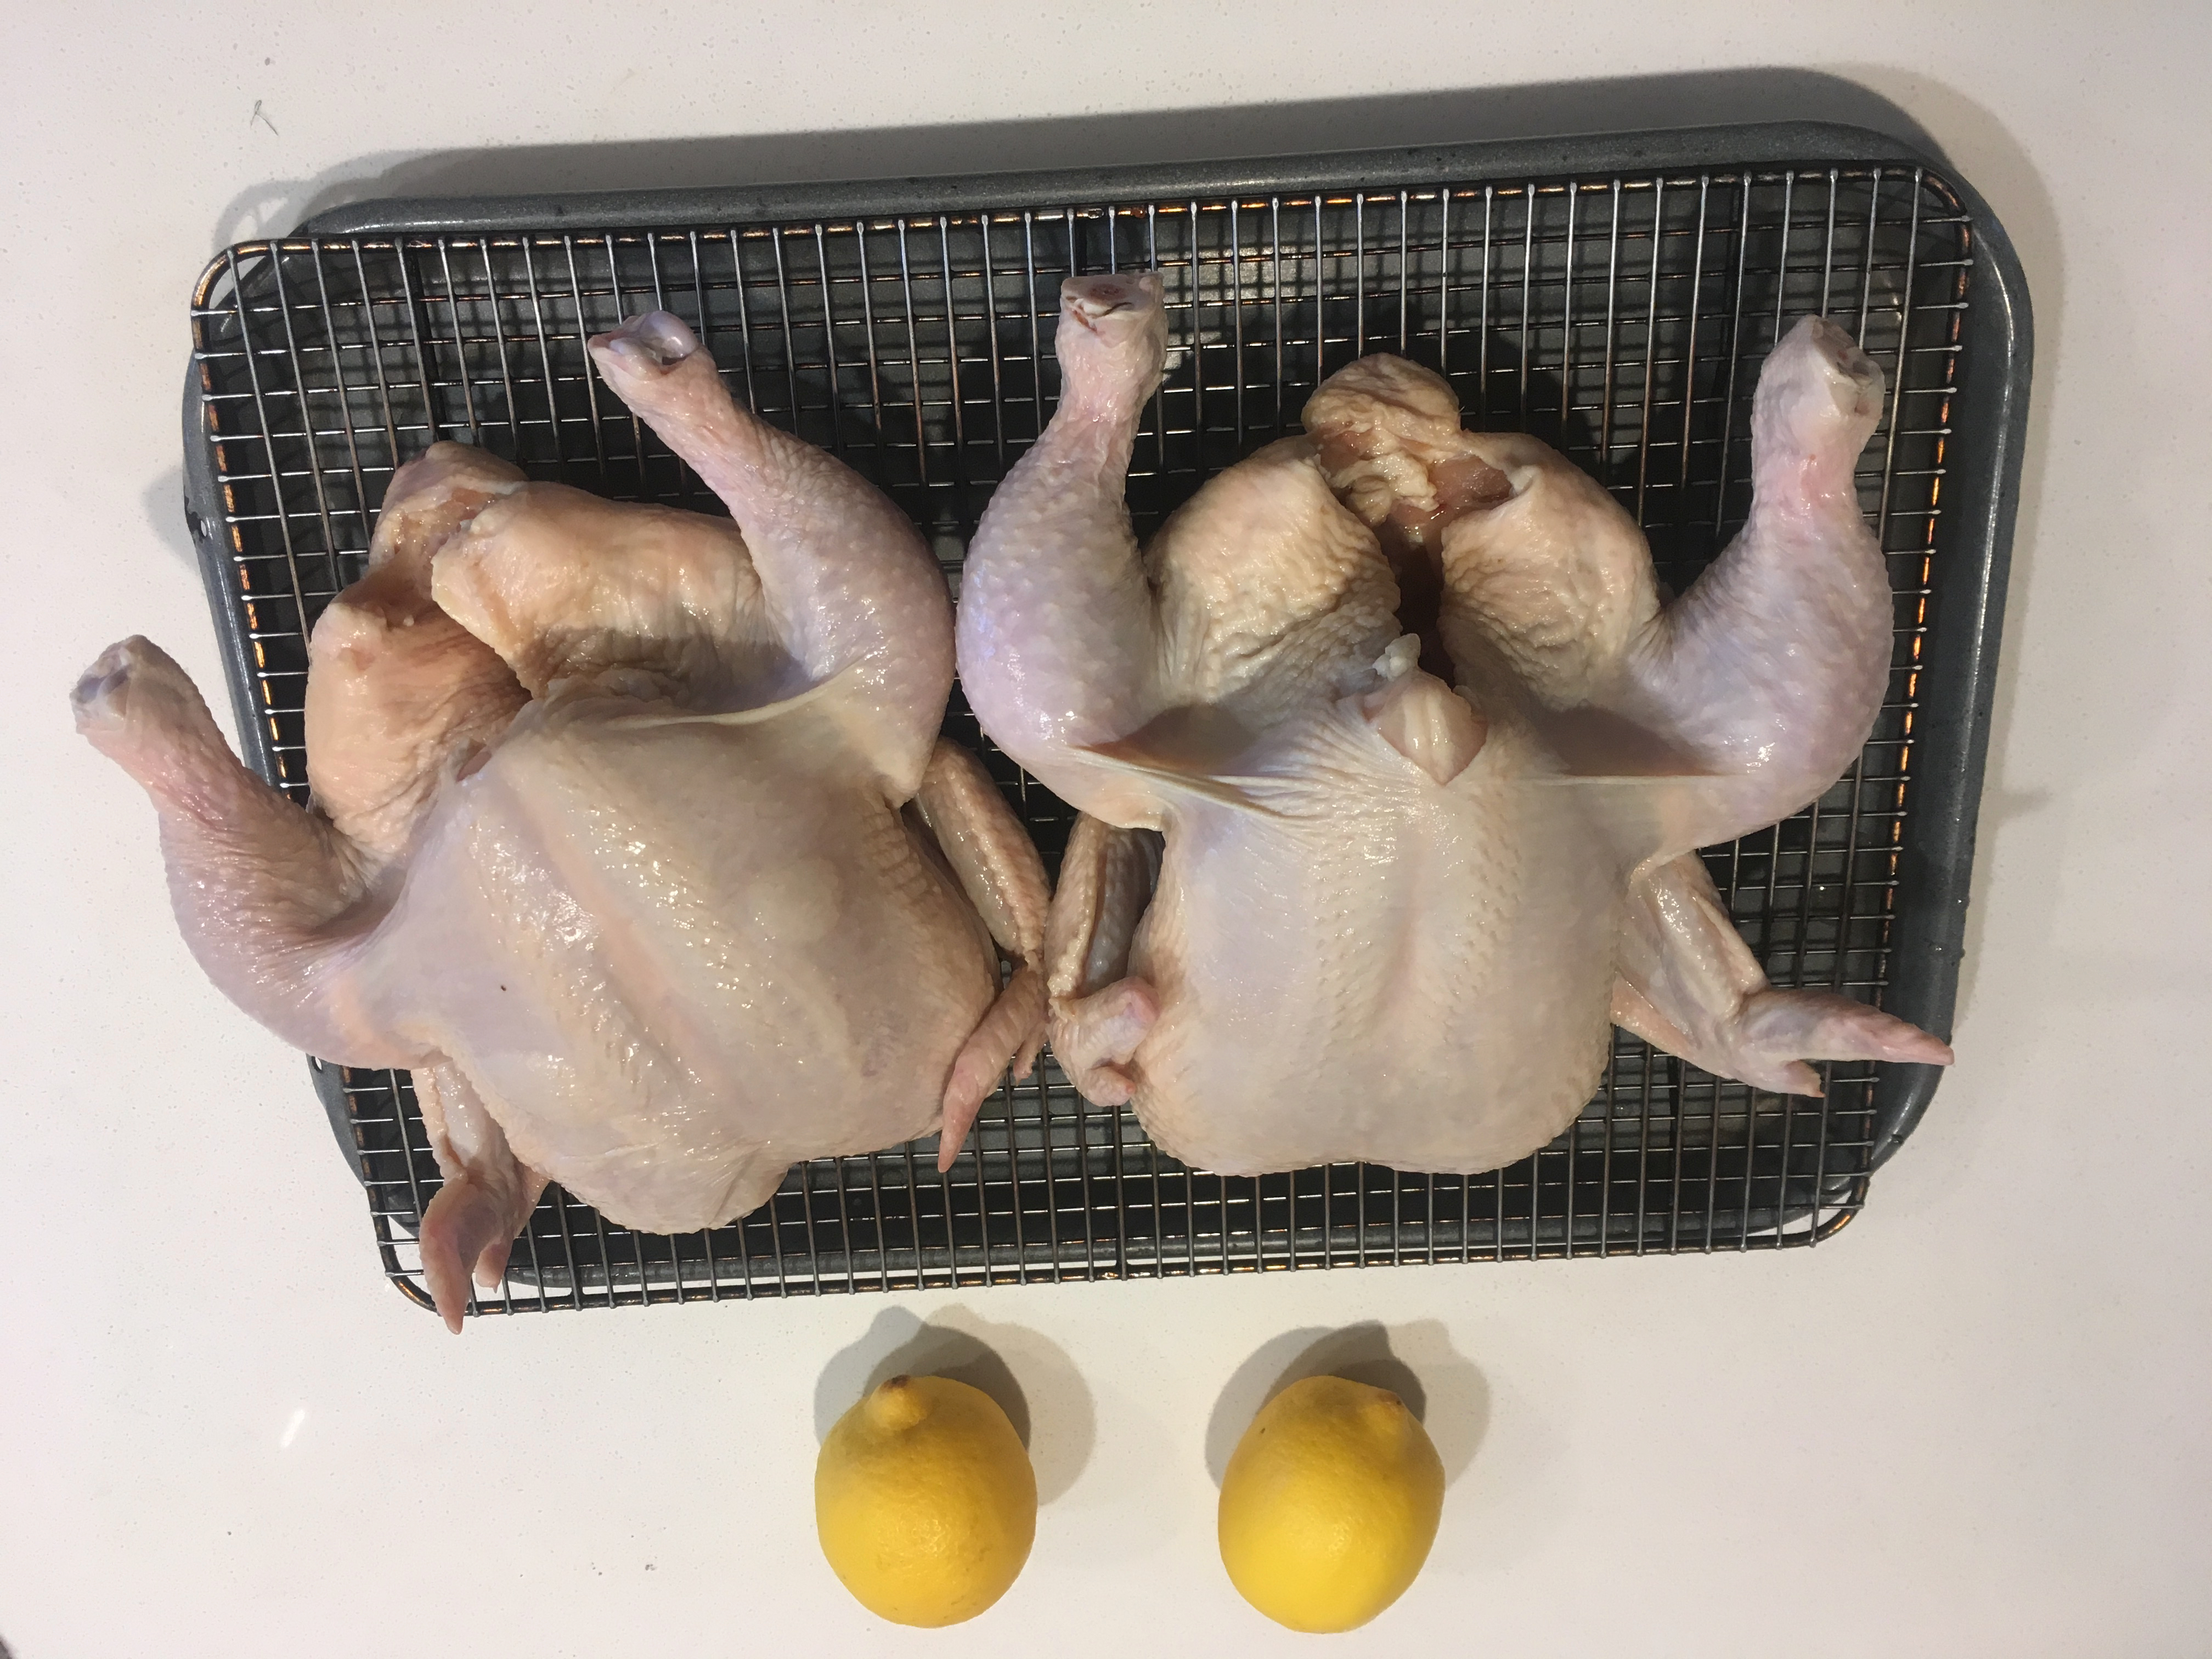
\includegraphics[width=0.25\textwidth]{\imageDir/\fileName/IMG_3197.jpg} &
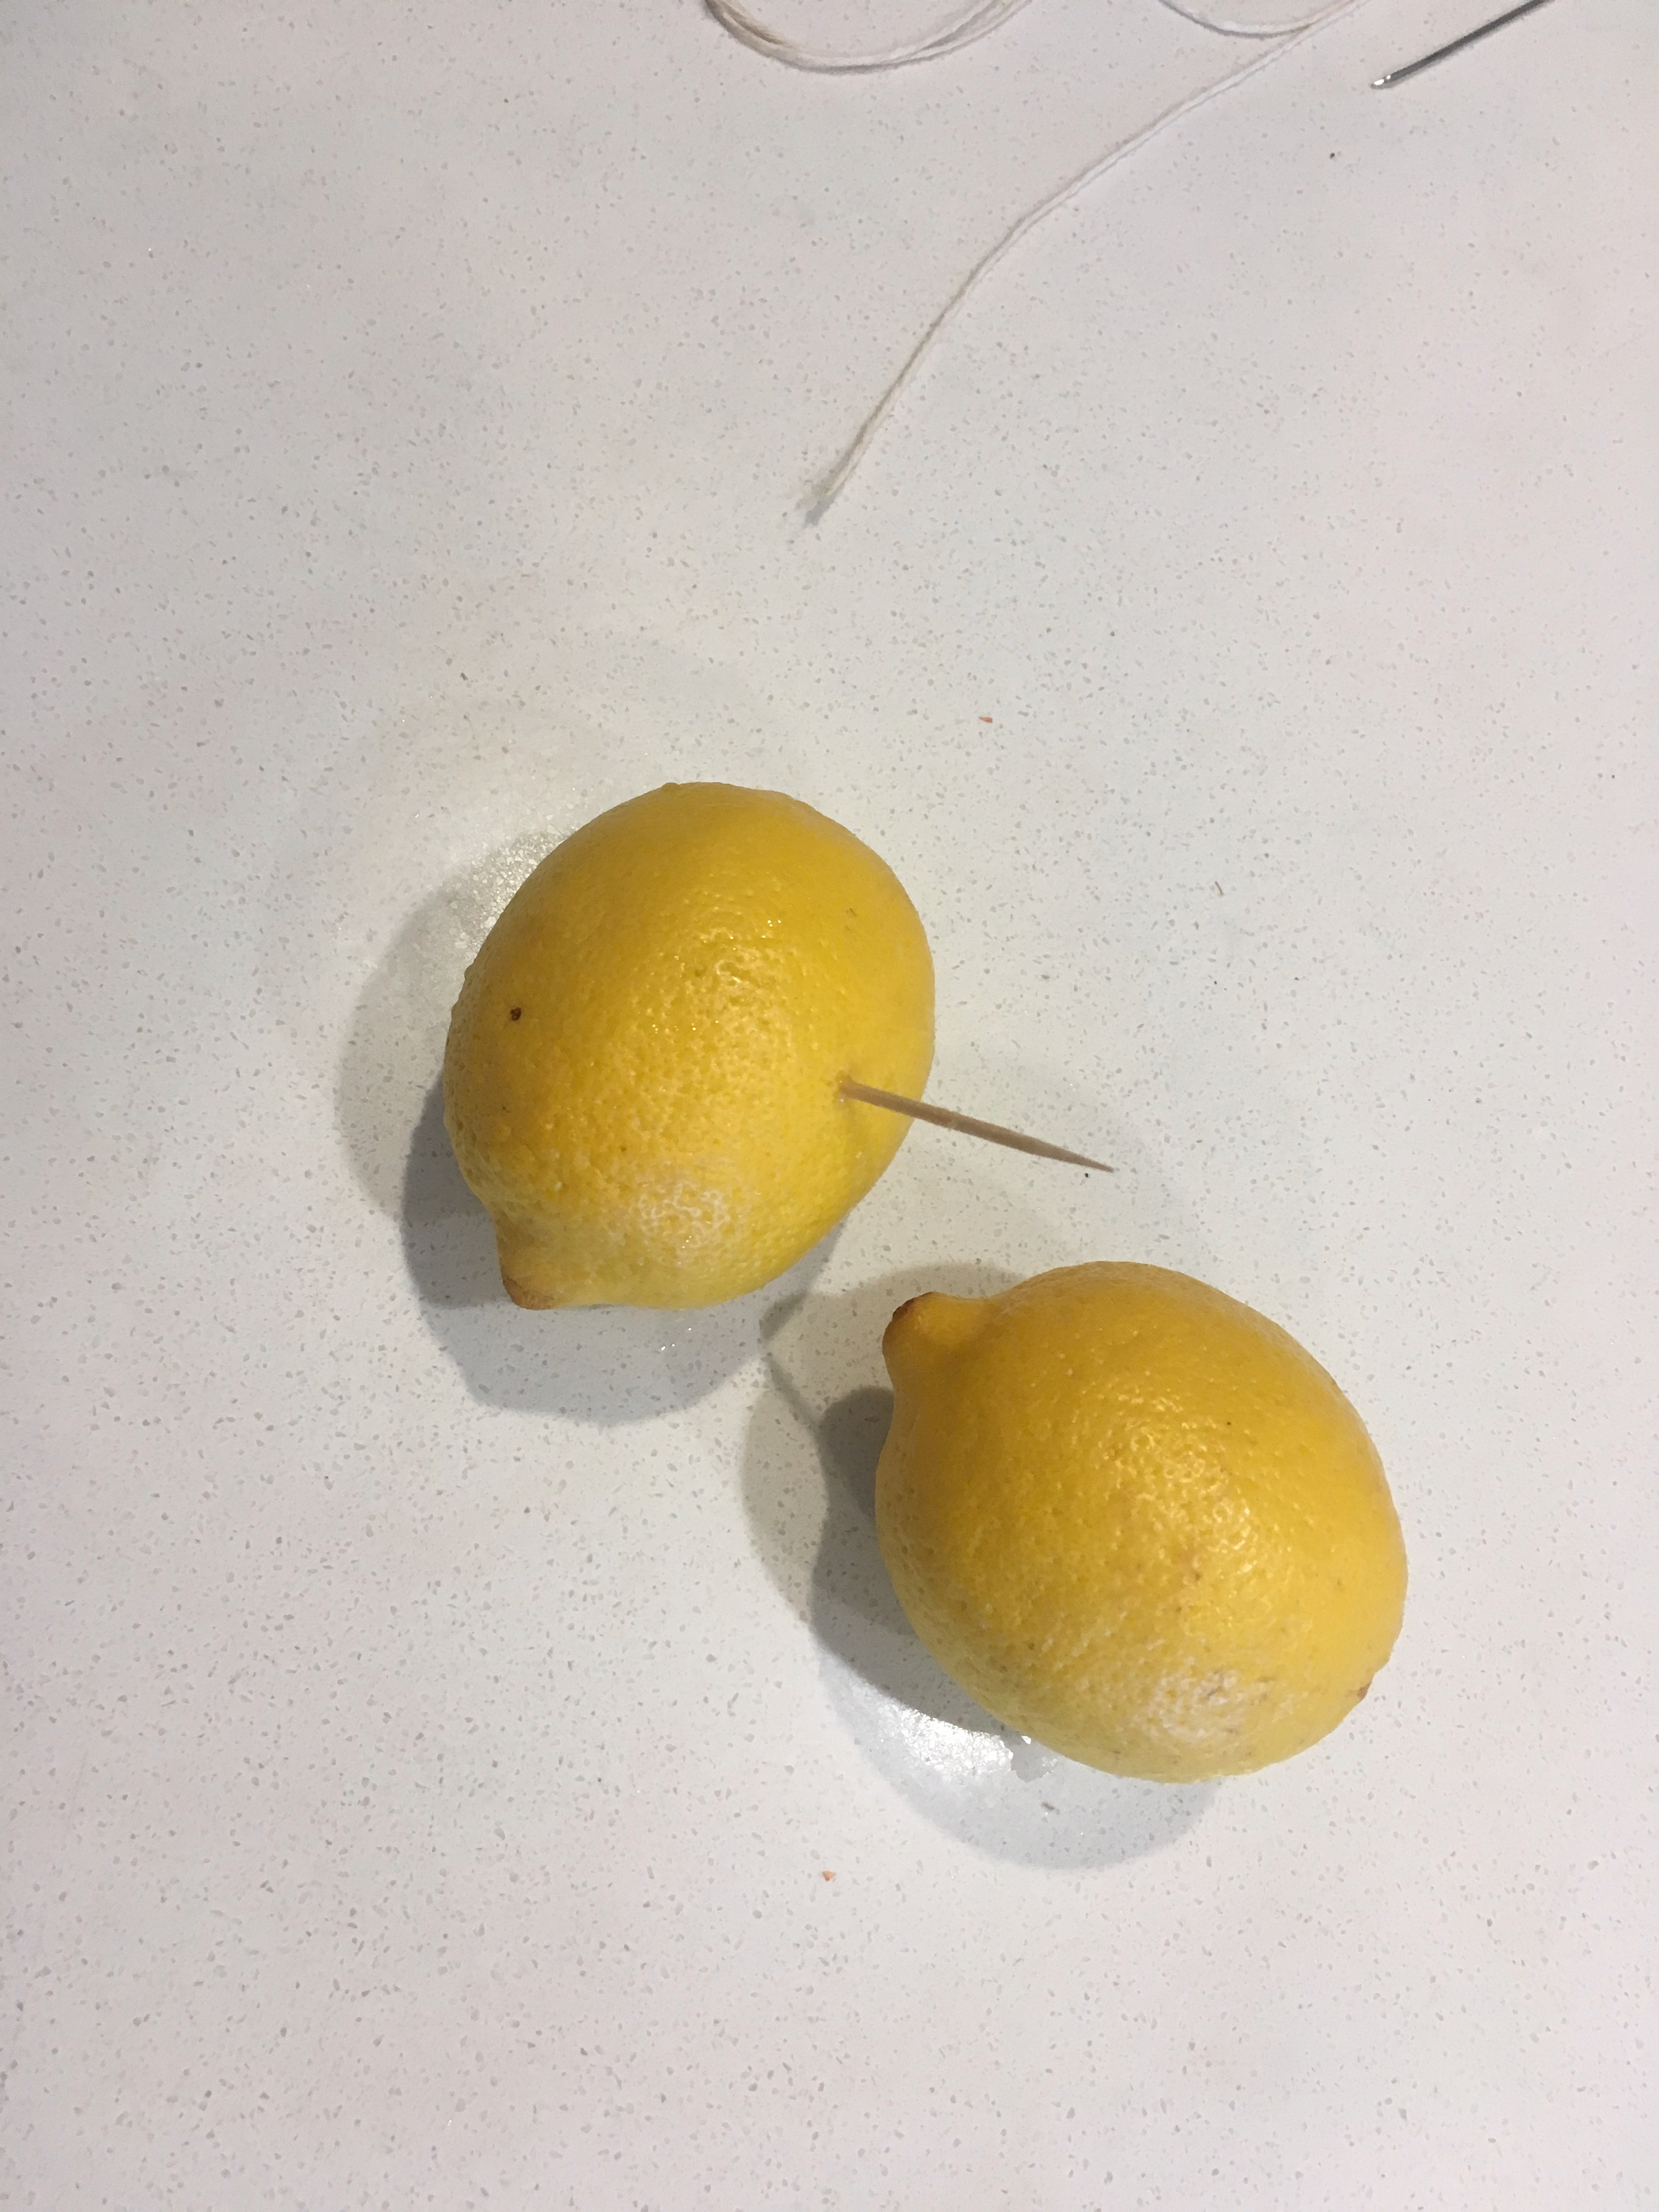
\includegraphics[width=0.25\textwidth]{\imageDir/\fileName/IMG_3212.jpg} &
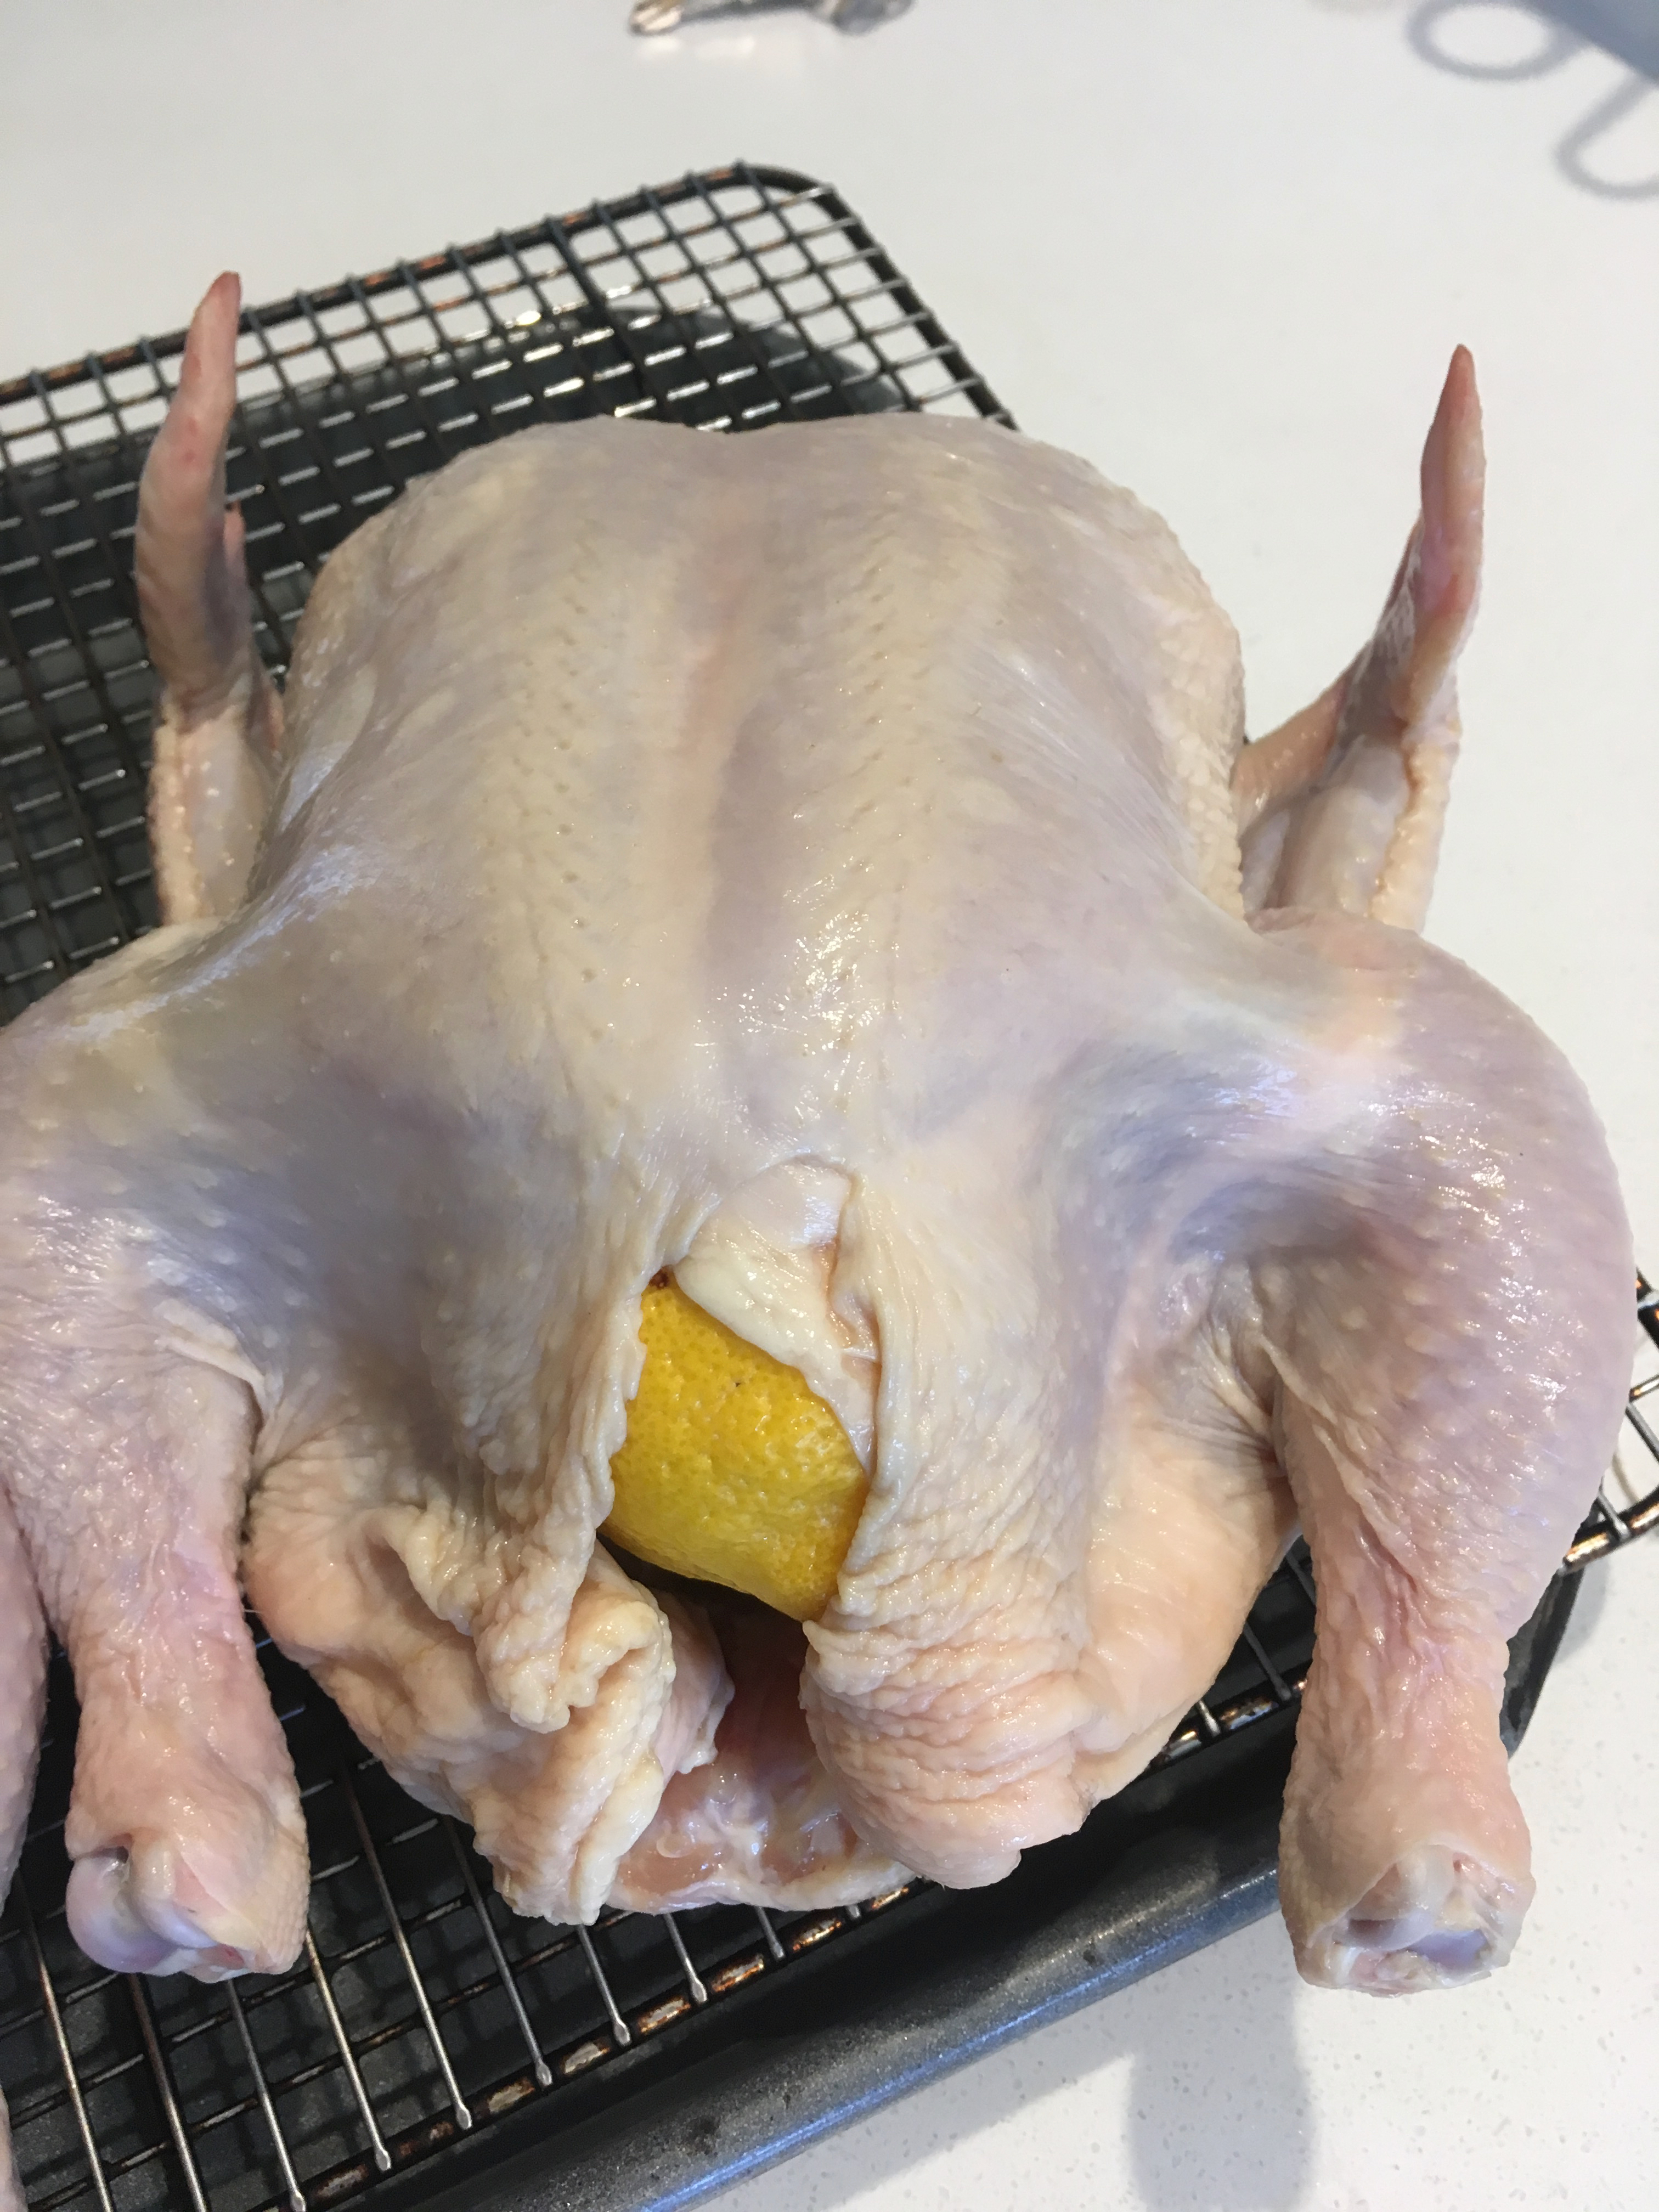
\includegraphics[width=0.25\textwidth]{\imageDir/\fileName/IMG_3213.jpg} \\
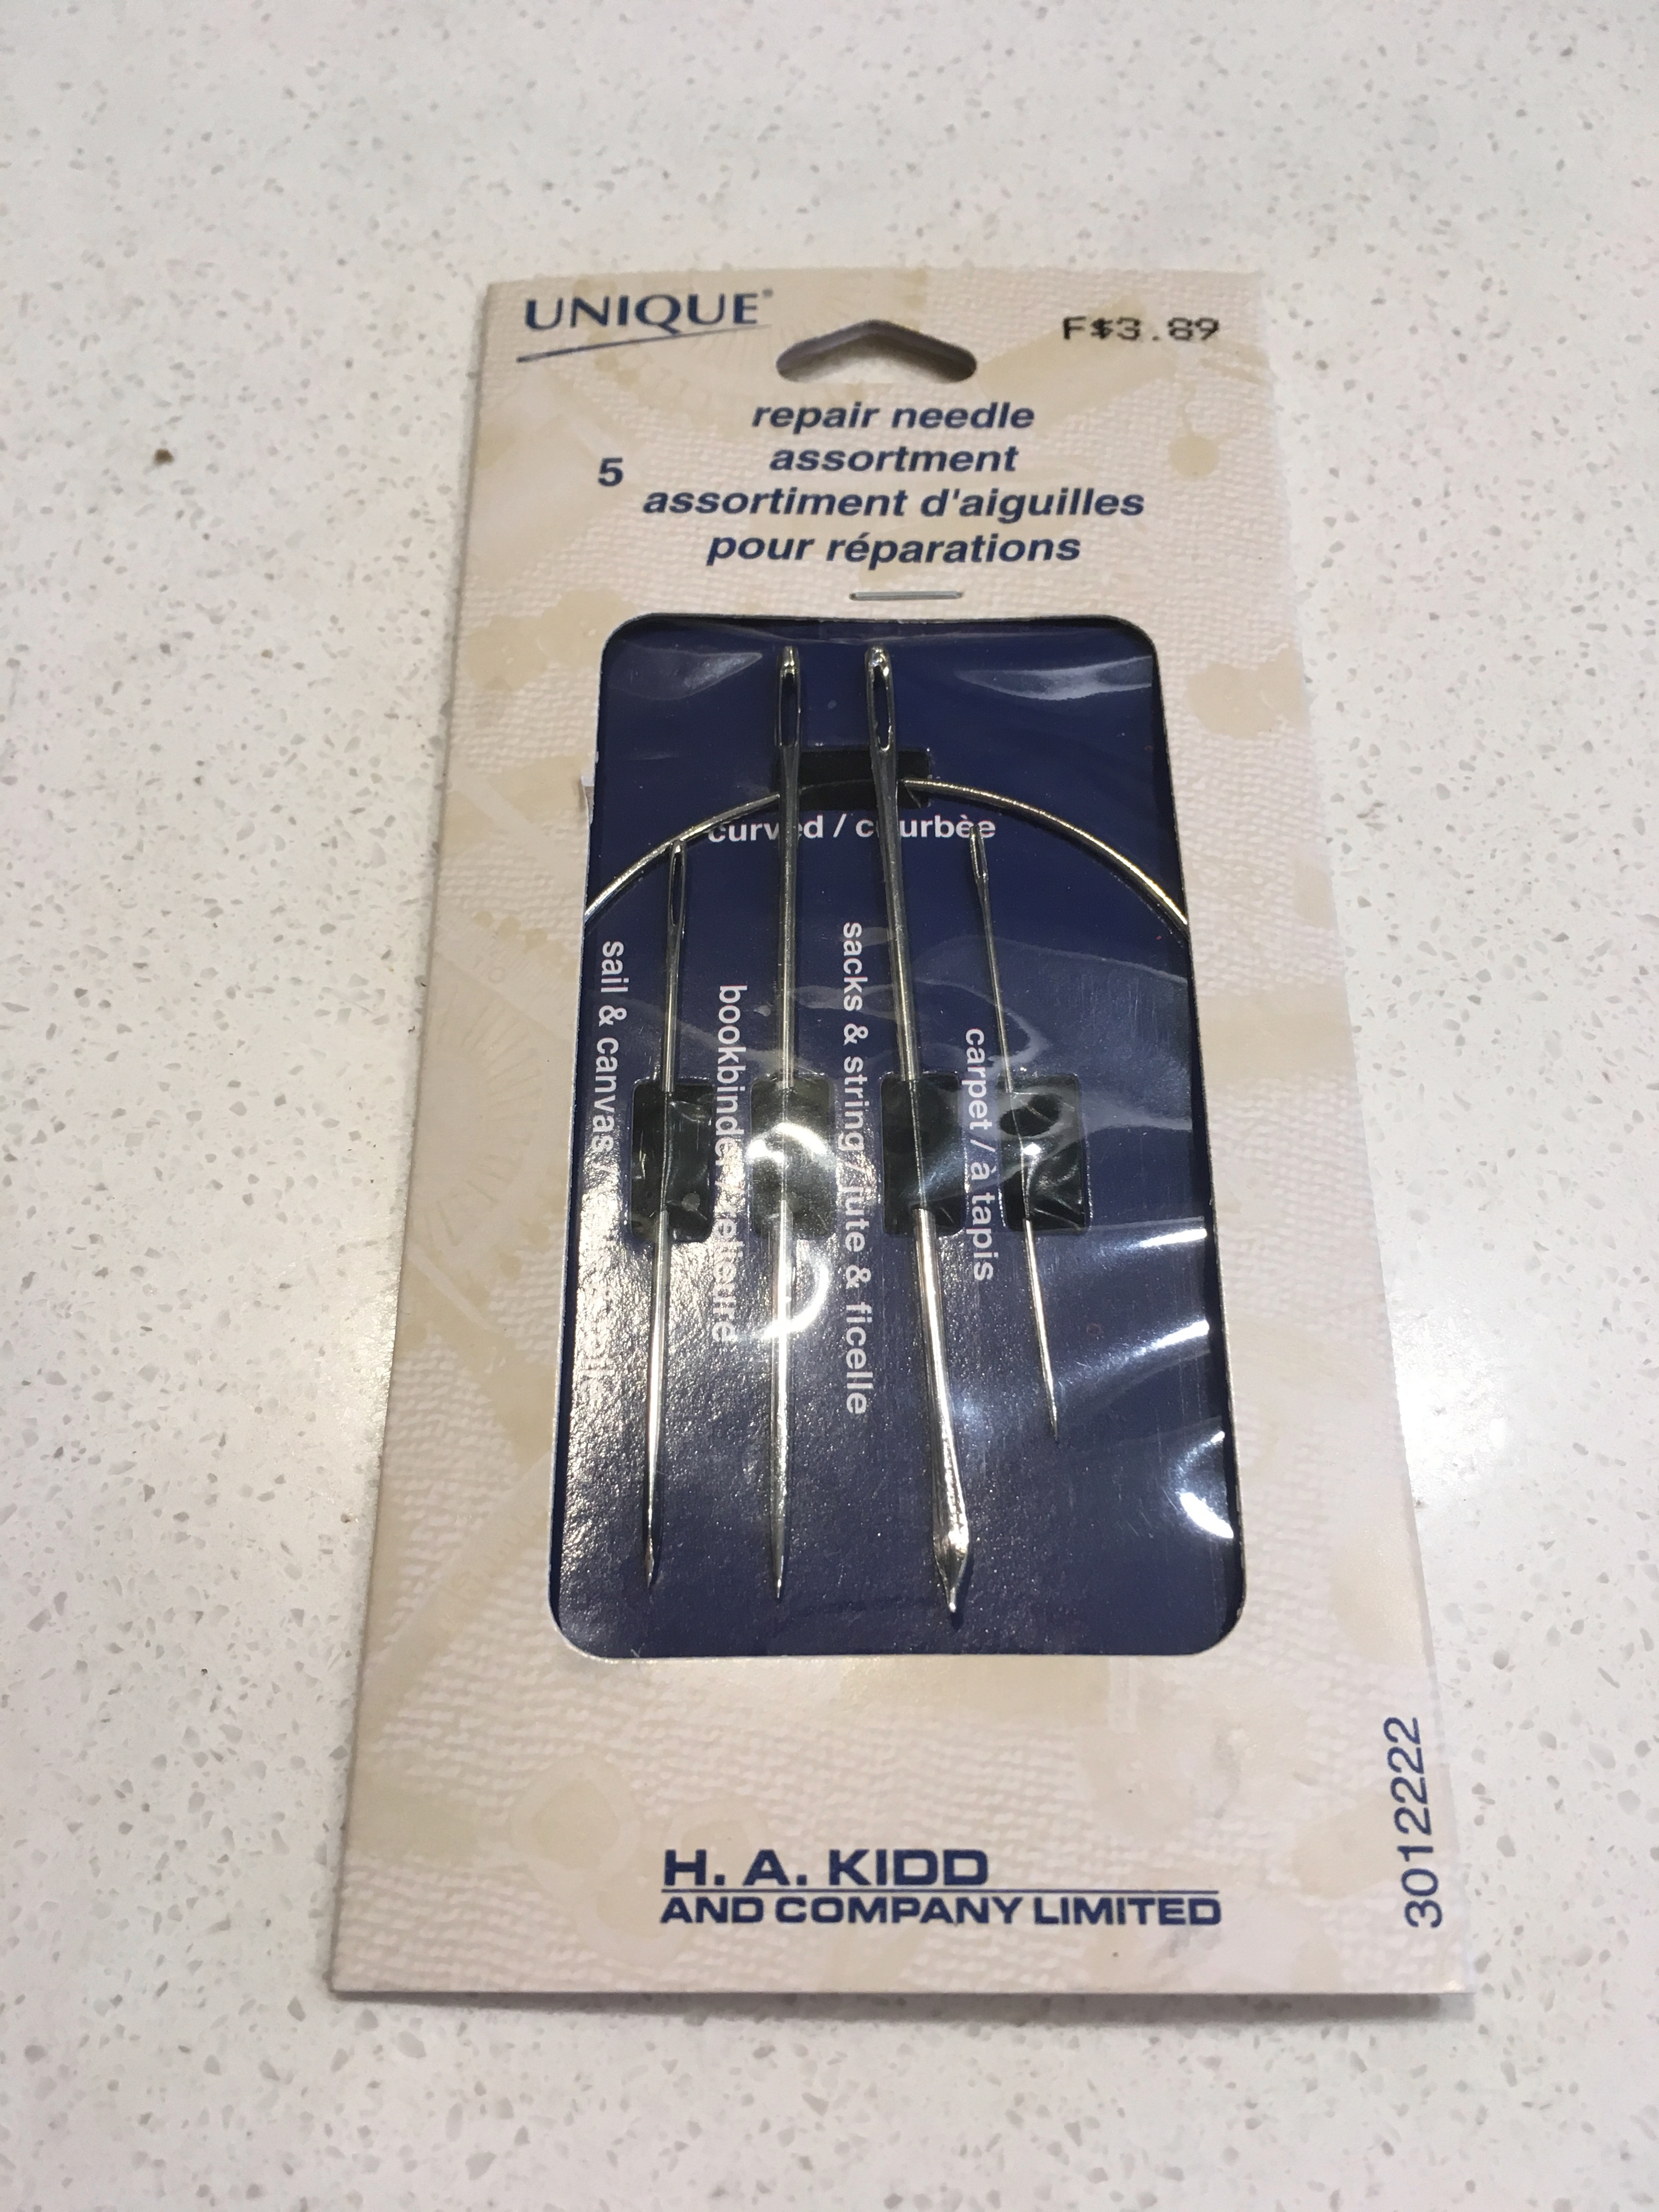
\includegraphics[width=0.25\textwidth]{\imageDir/\fileName/IMG_3206.jpg} &
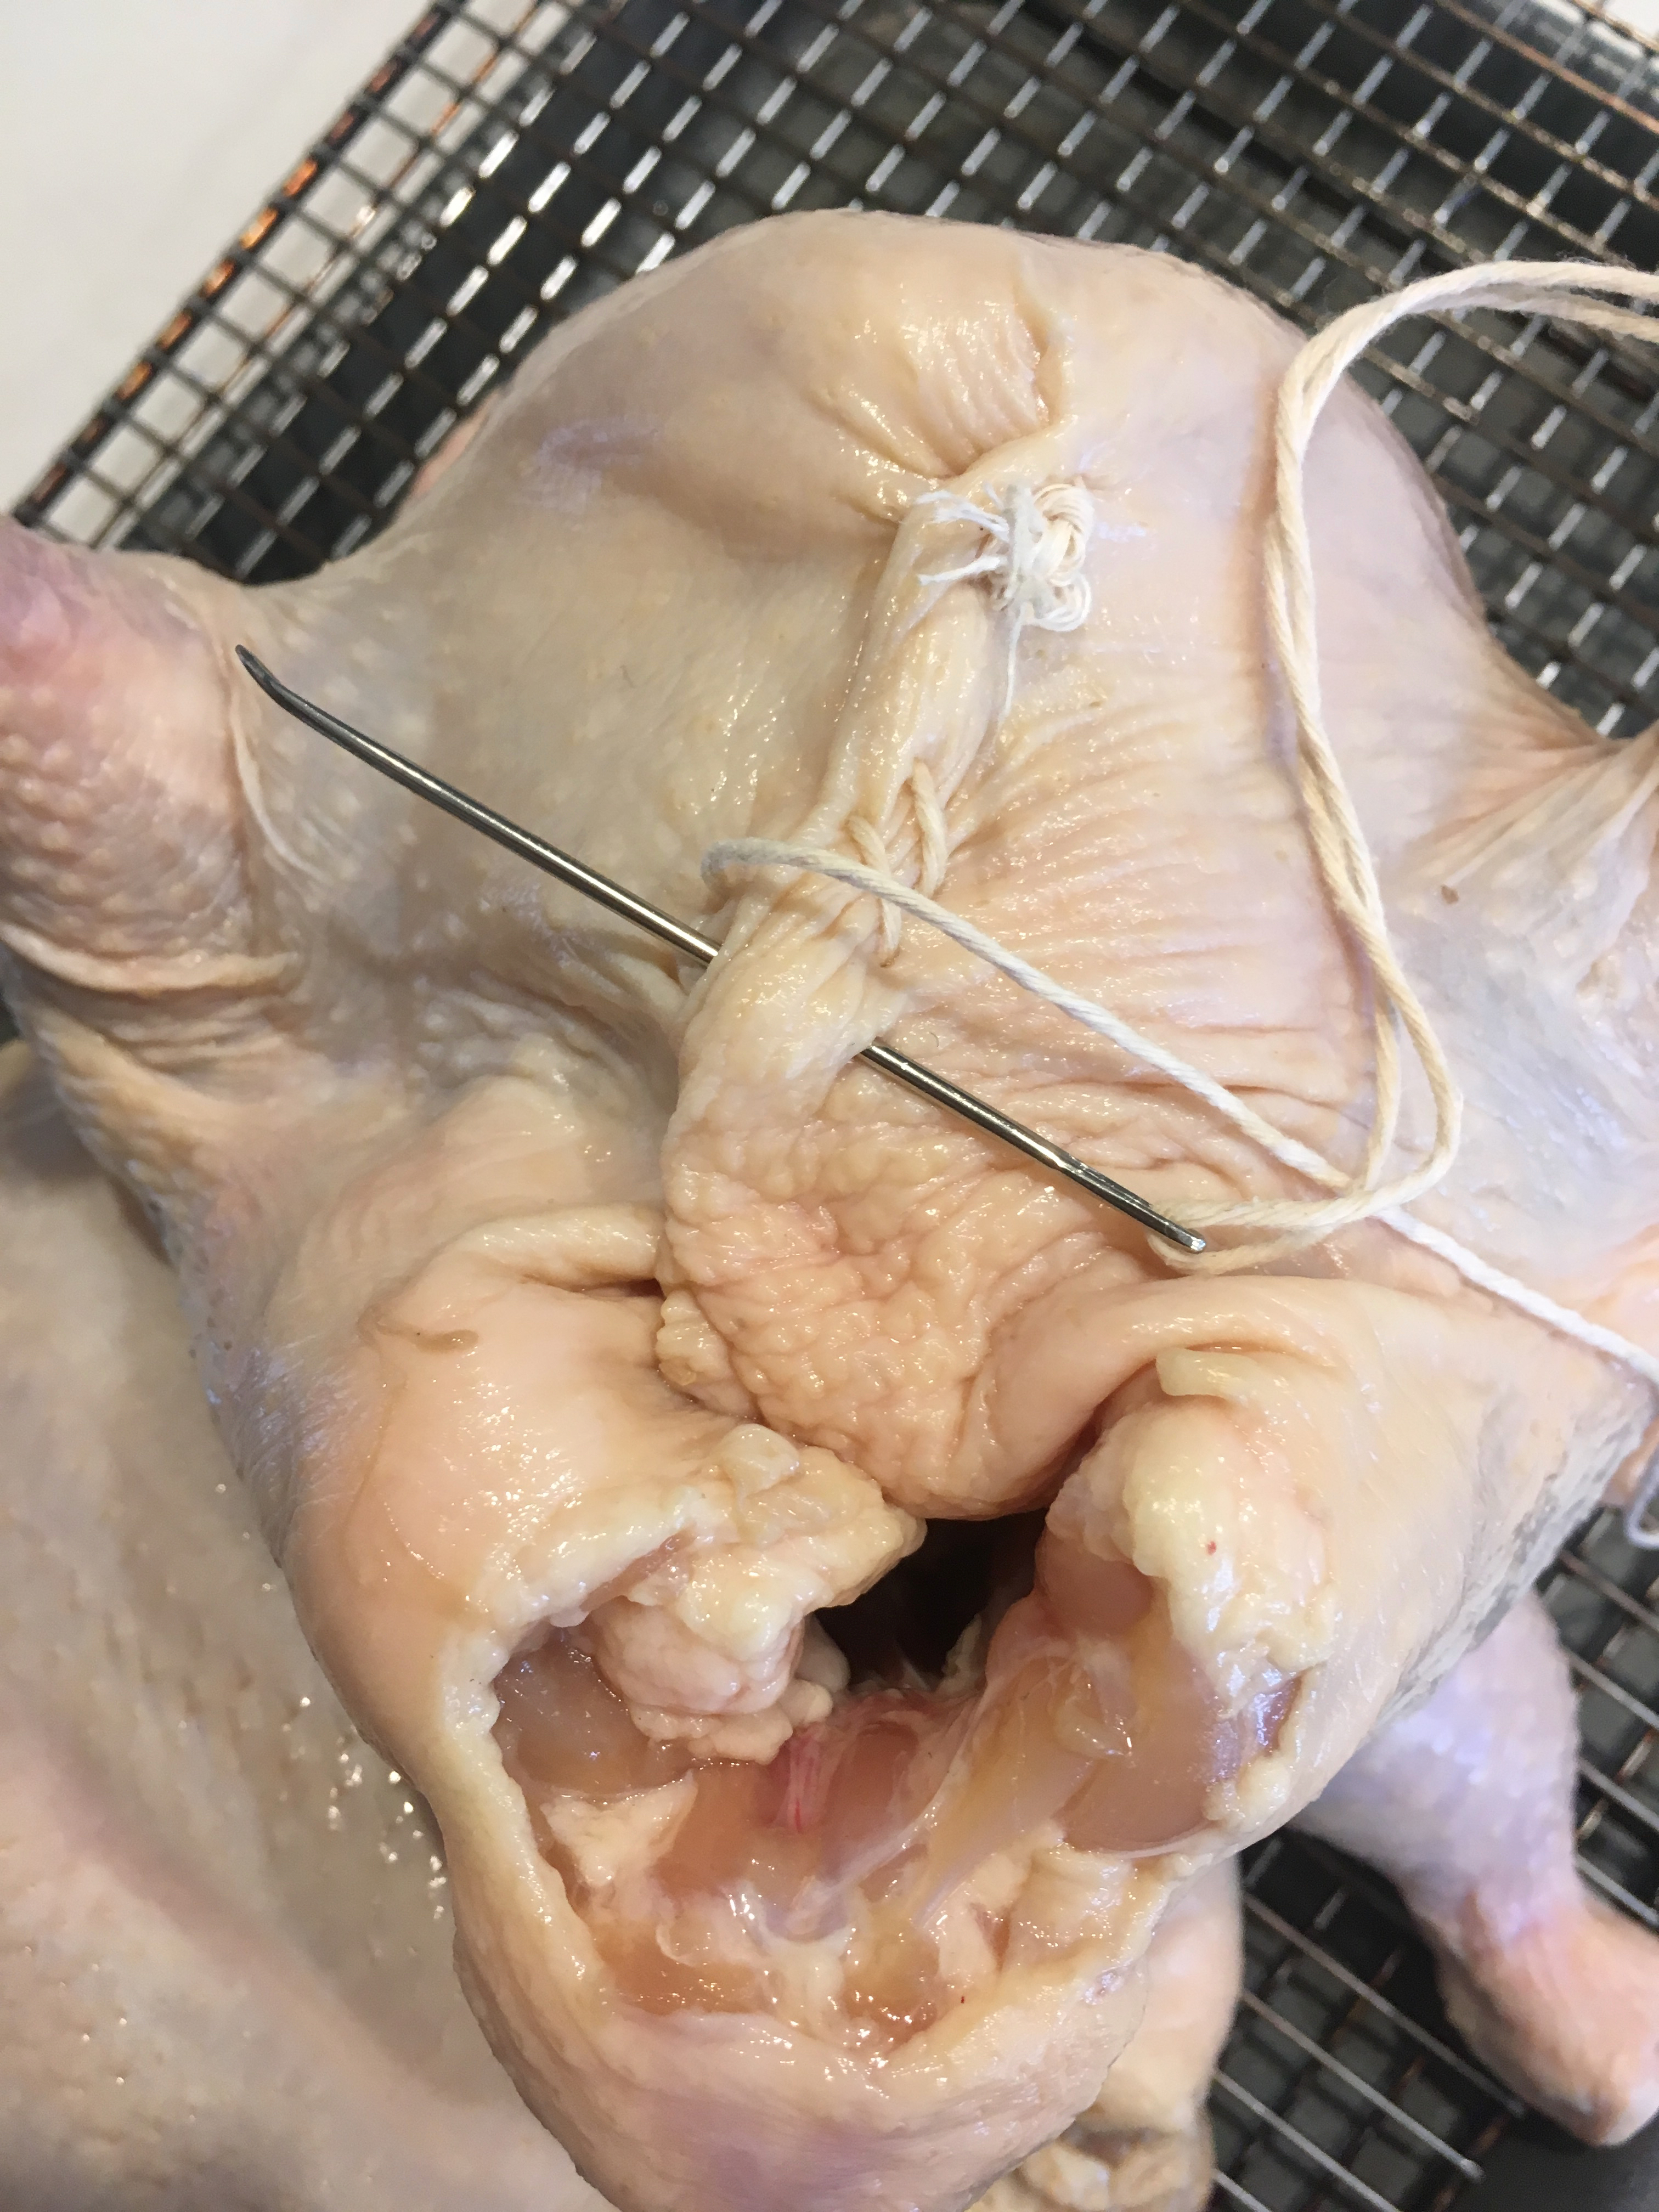
\includegraphics[width=0.25\textwidth]{\imageDir/\fileName/IMG_3214.jpg} &
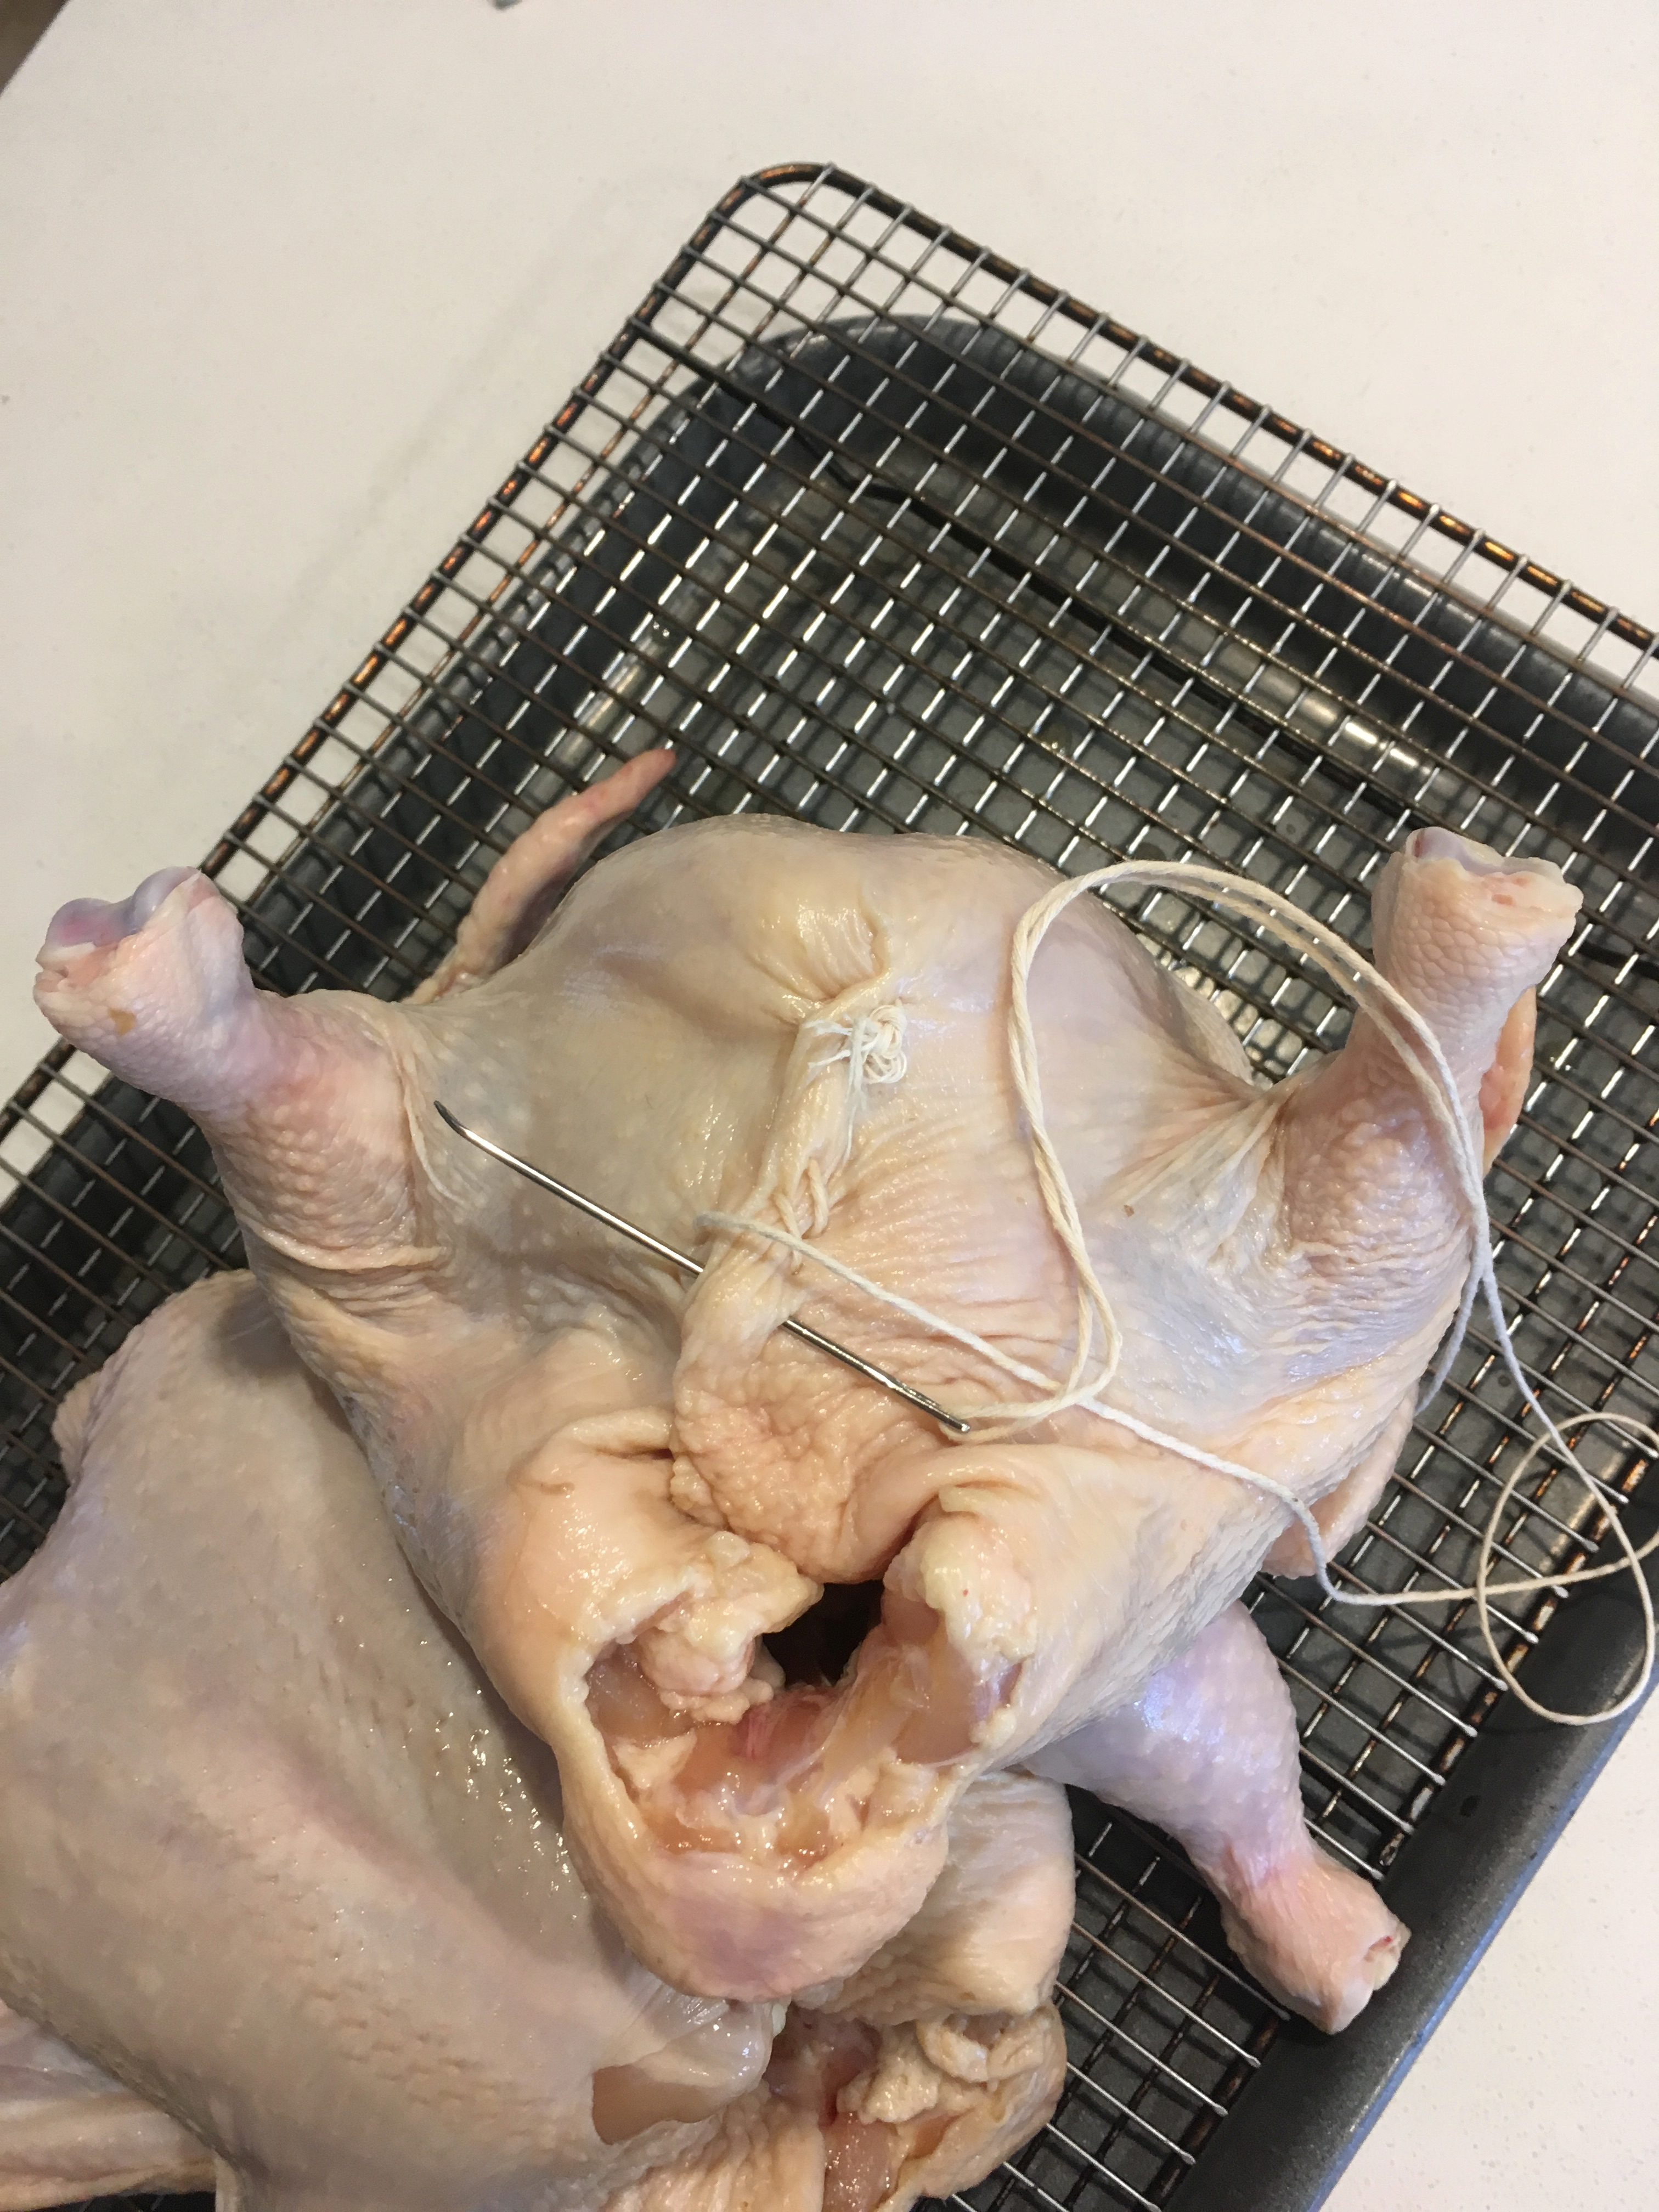
\includegraphics[width=0.25\textwidth]{\imageDir/\fileName/IMG_3216.jpg} \\
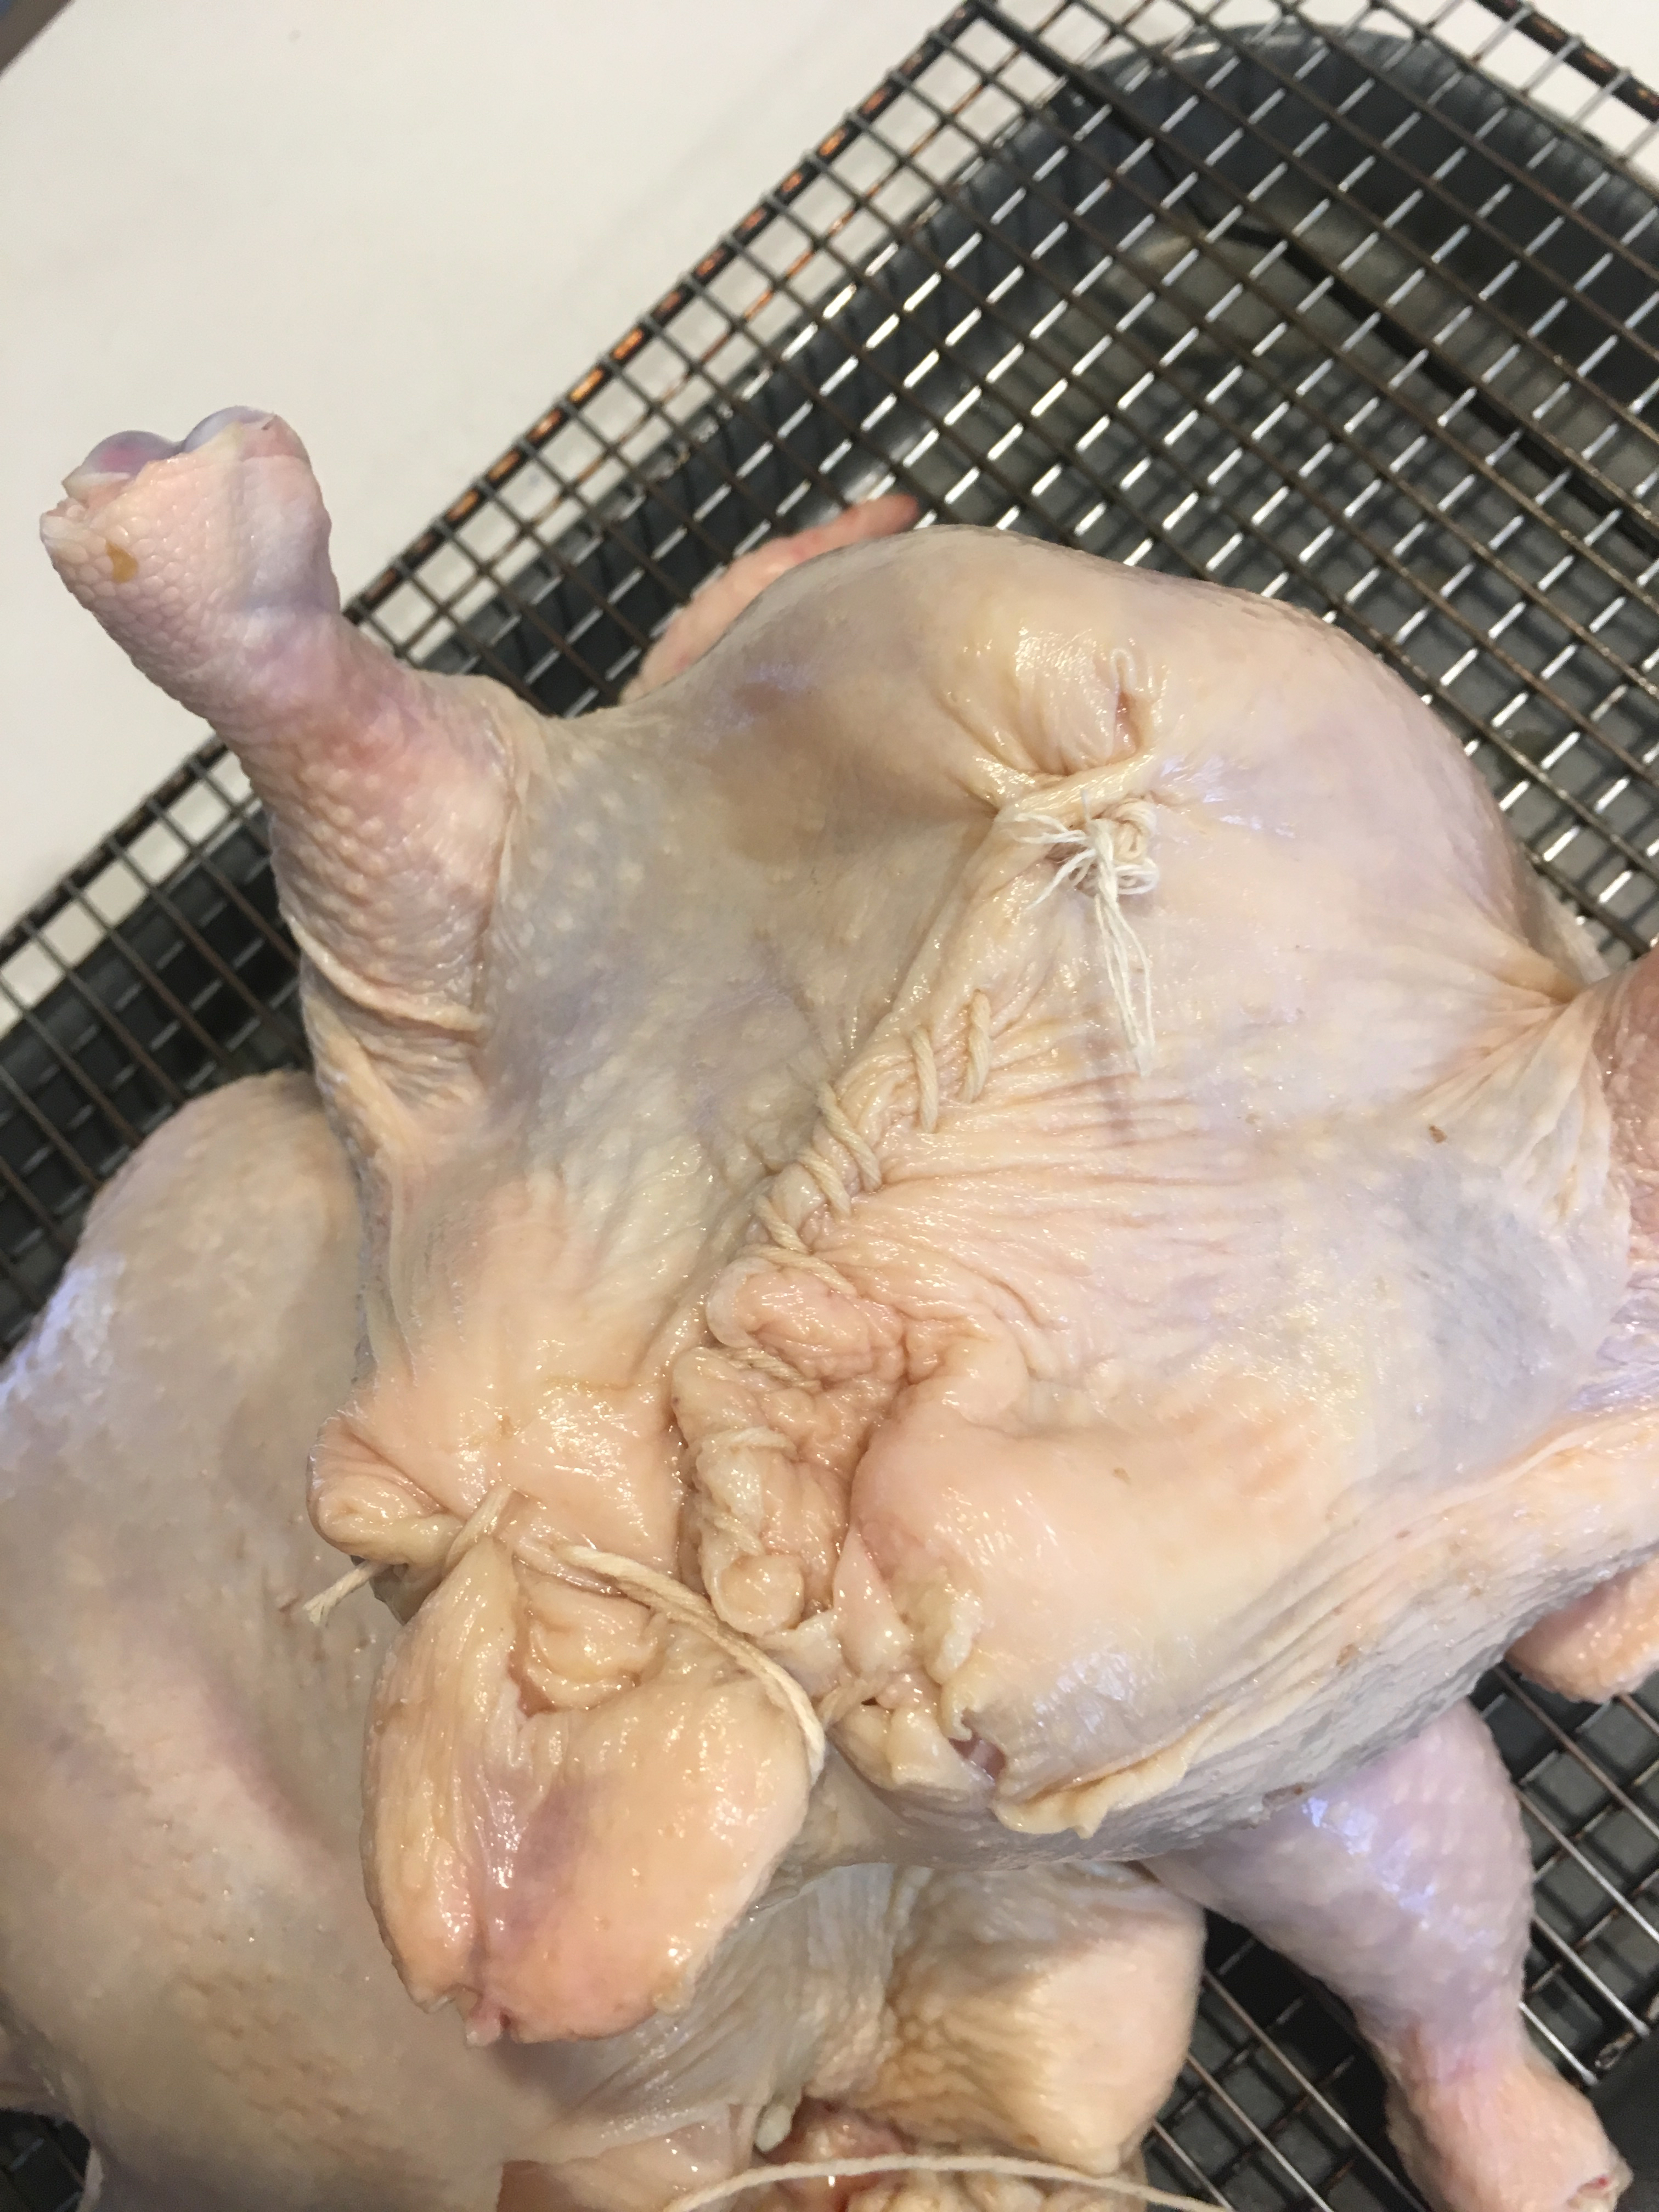
\includegraphics[width=0.25\textwidth]{\imageDir/\fileName/IMG_3217.jpg} &
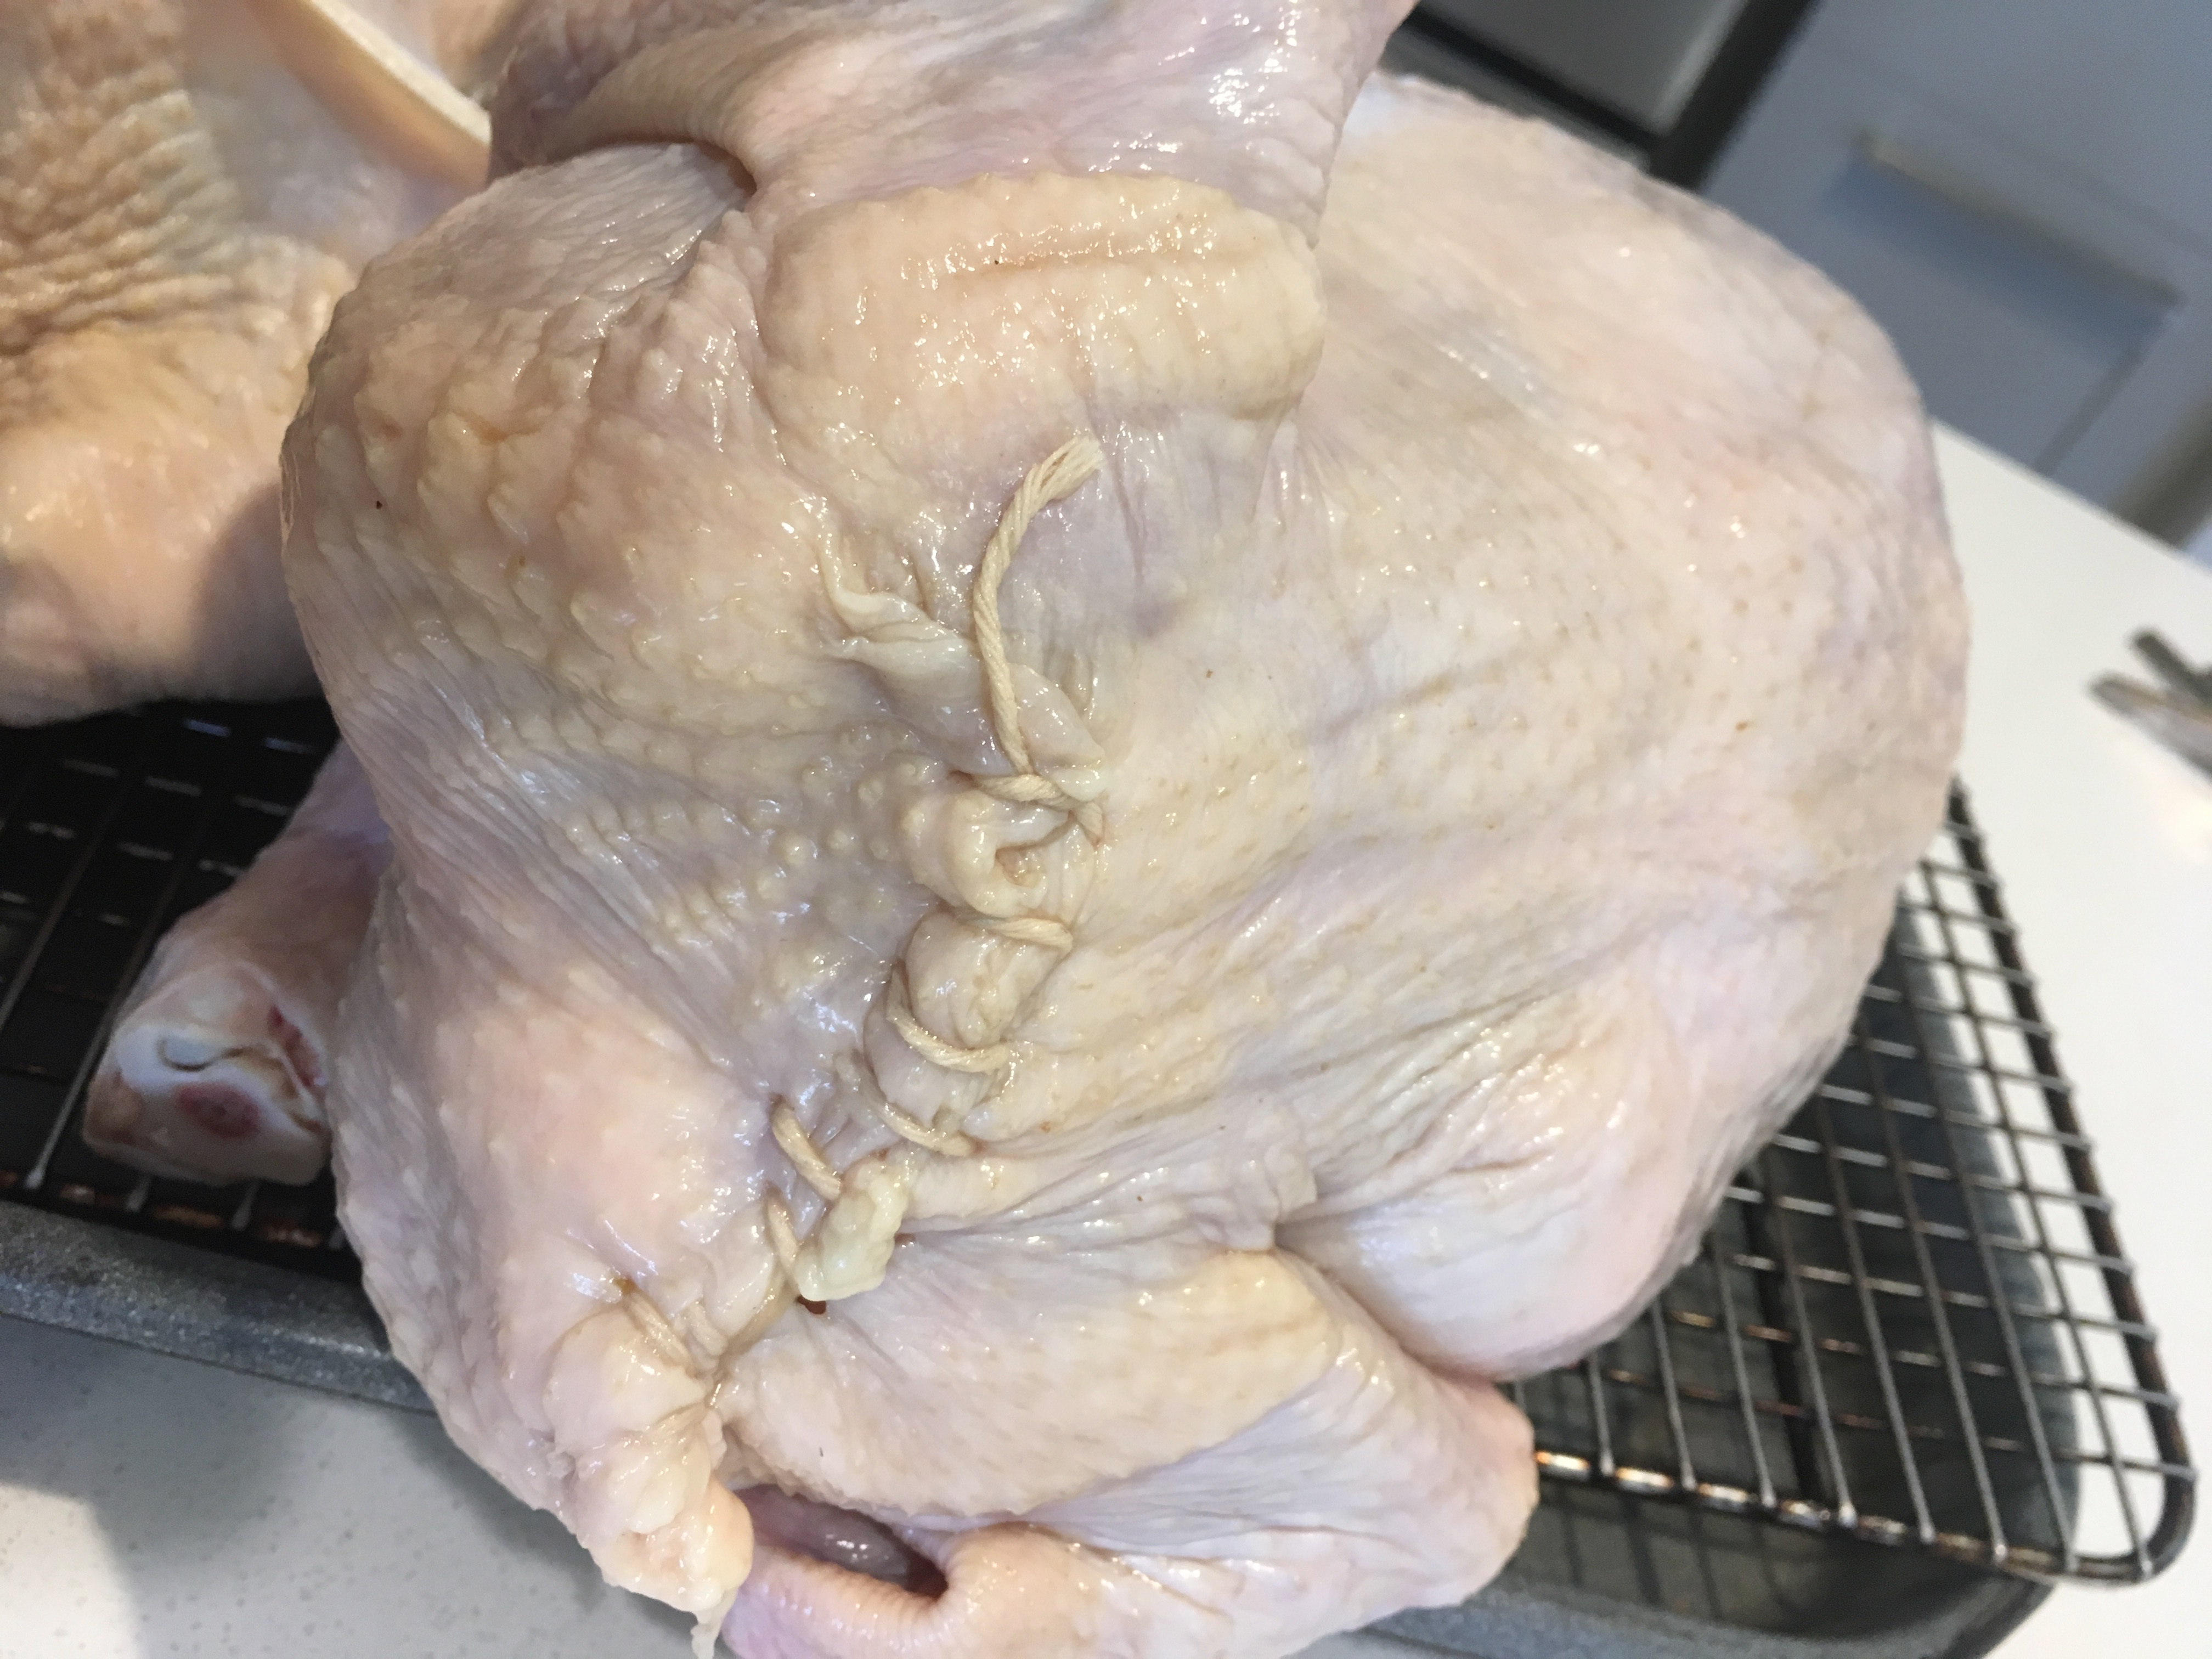
\includegraphics[width=0.25\textwidth]{\imageDir/\fileName/IMG_3218.jpg} &
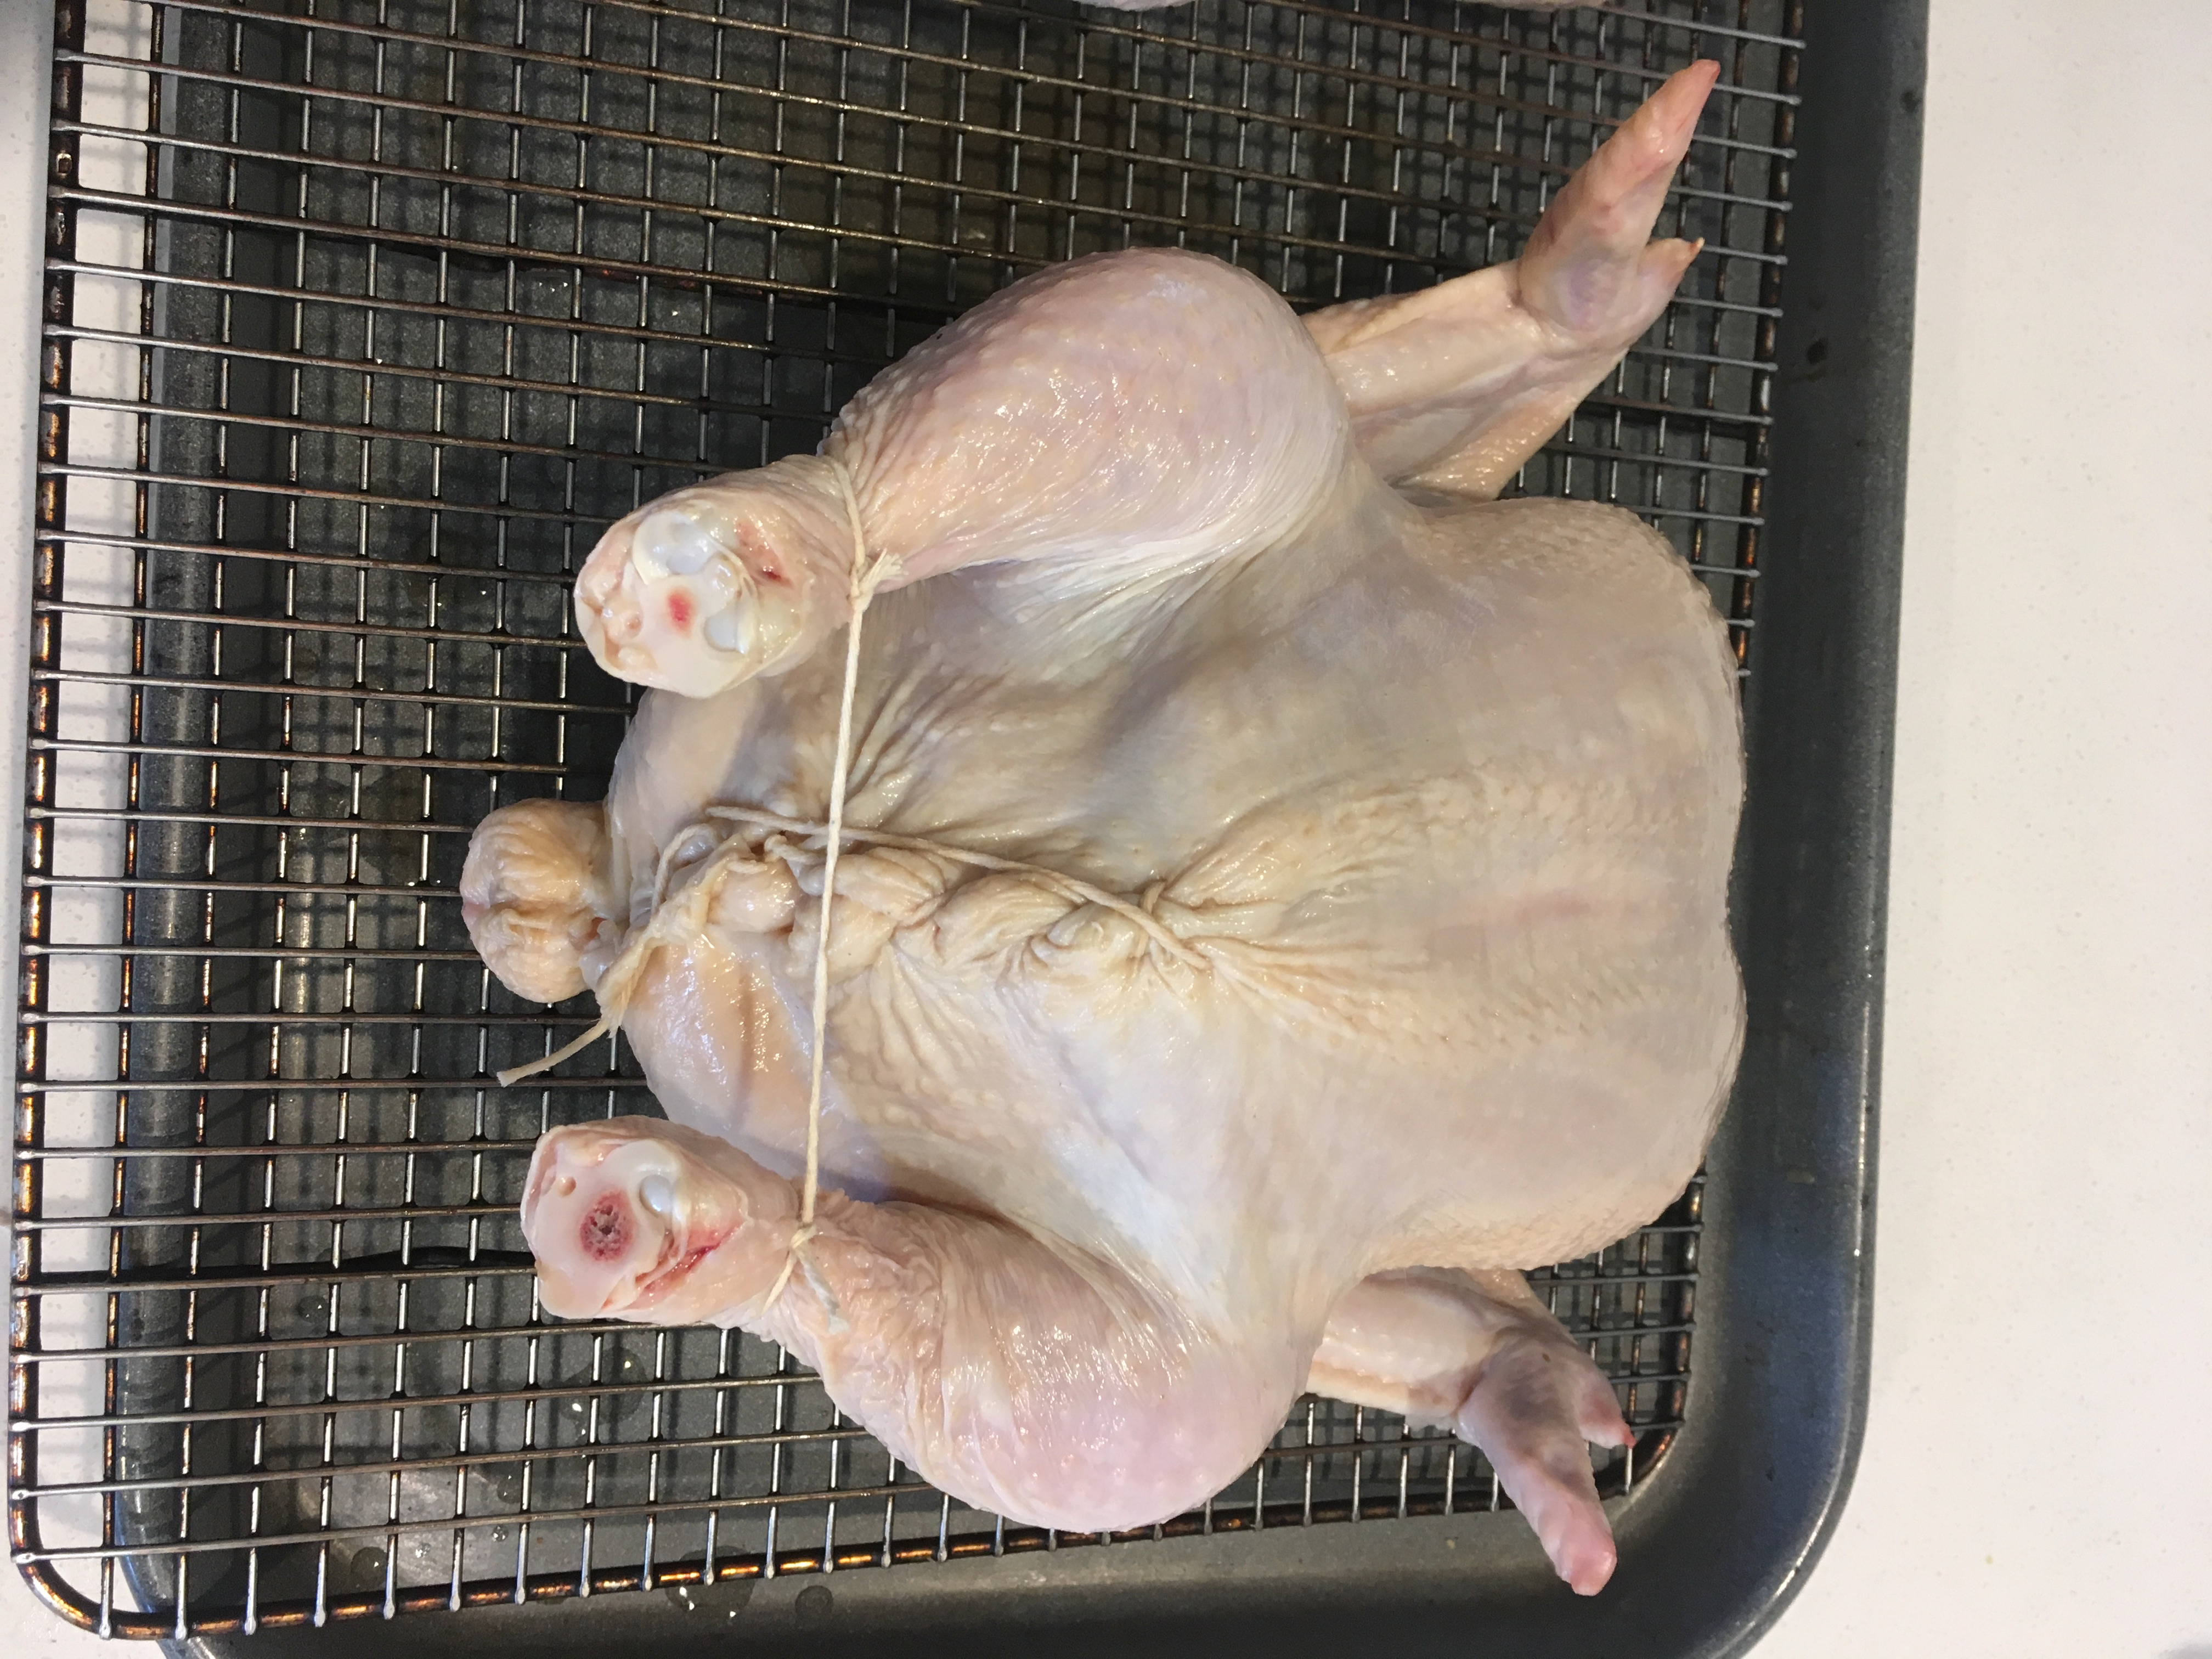
\includegraphics[width=0.25\textwidth]{\imageDir/\fileName/IMG_3219.jpg} \\
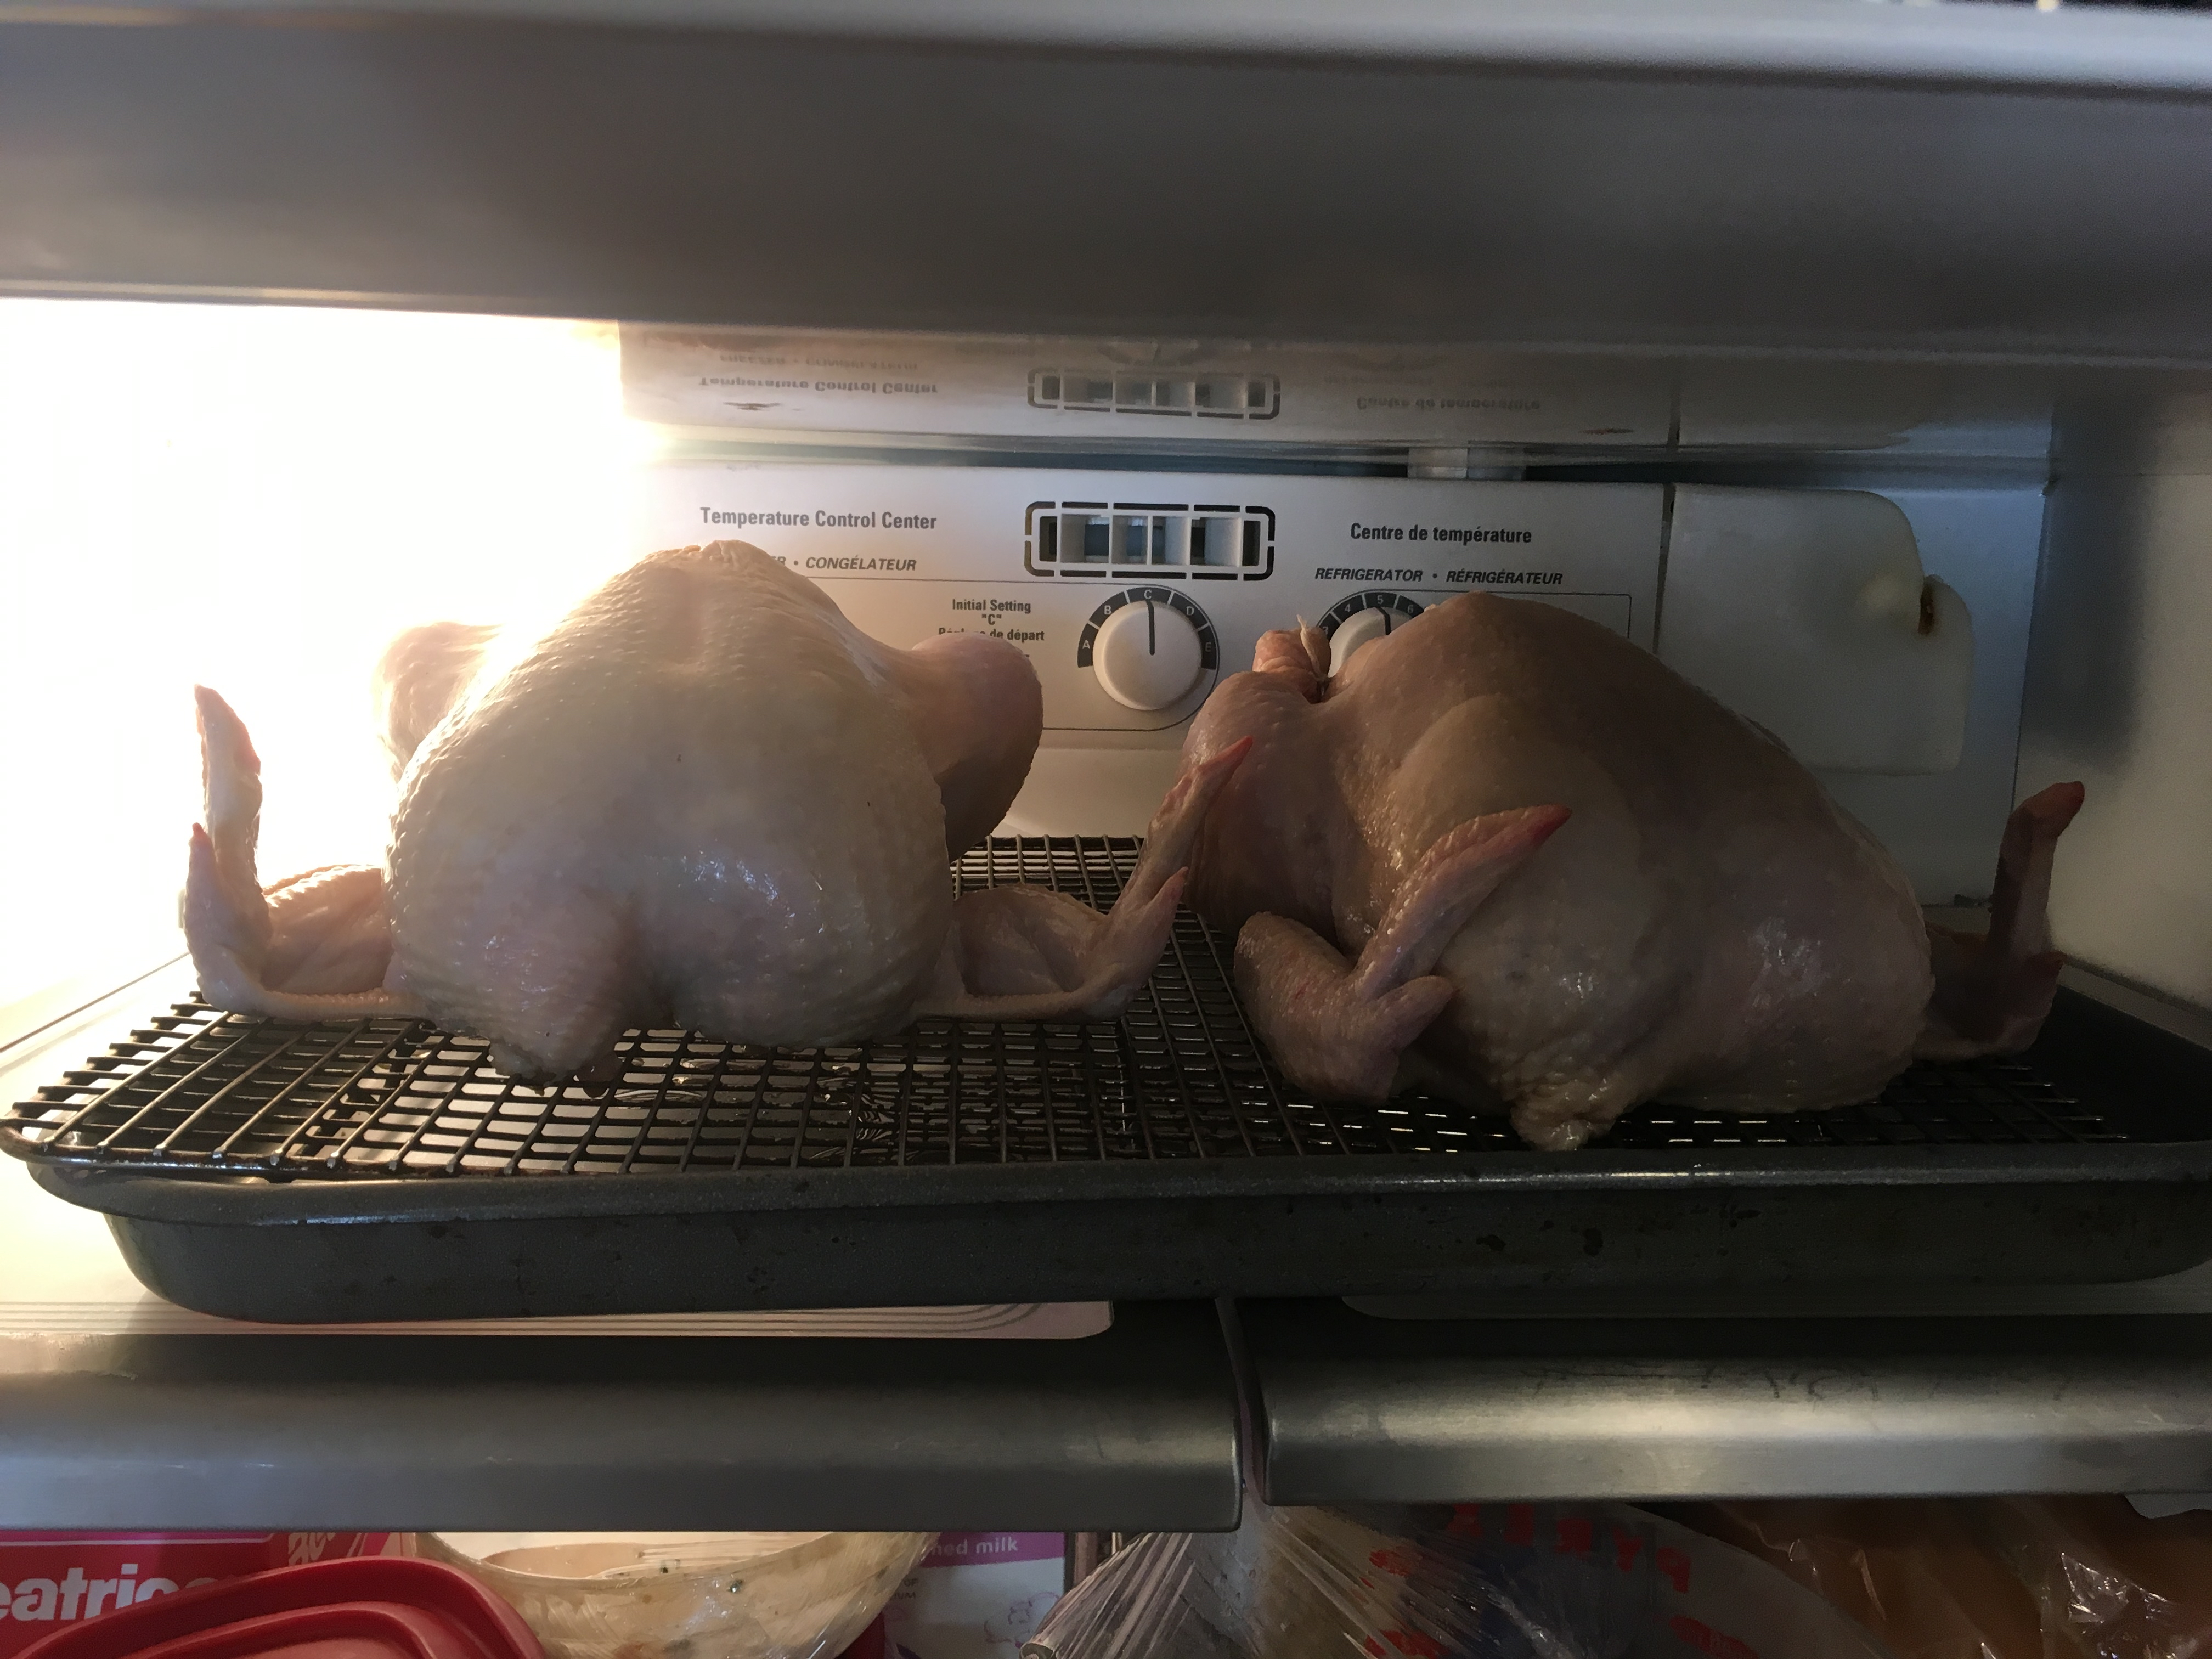
\includegraphics[width=0.25\textwidth]{\imageDir/\fileName/IMG_3220.jpg} &
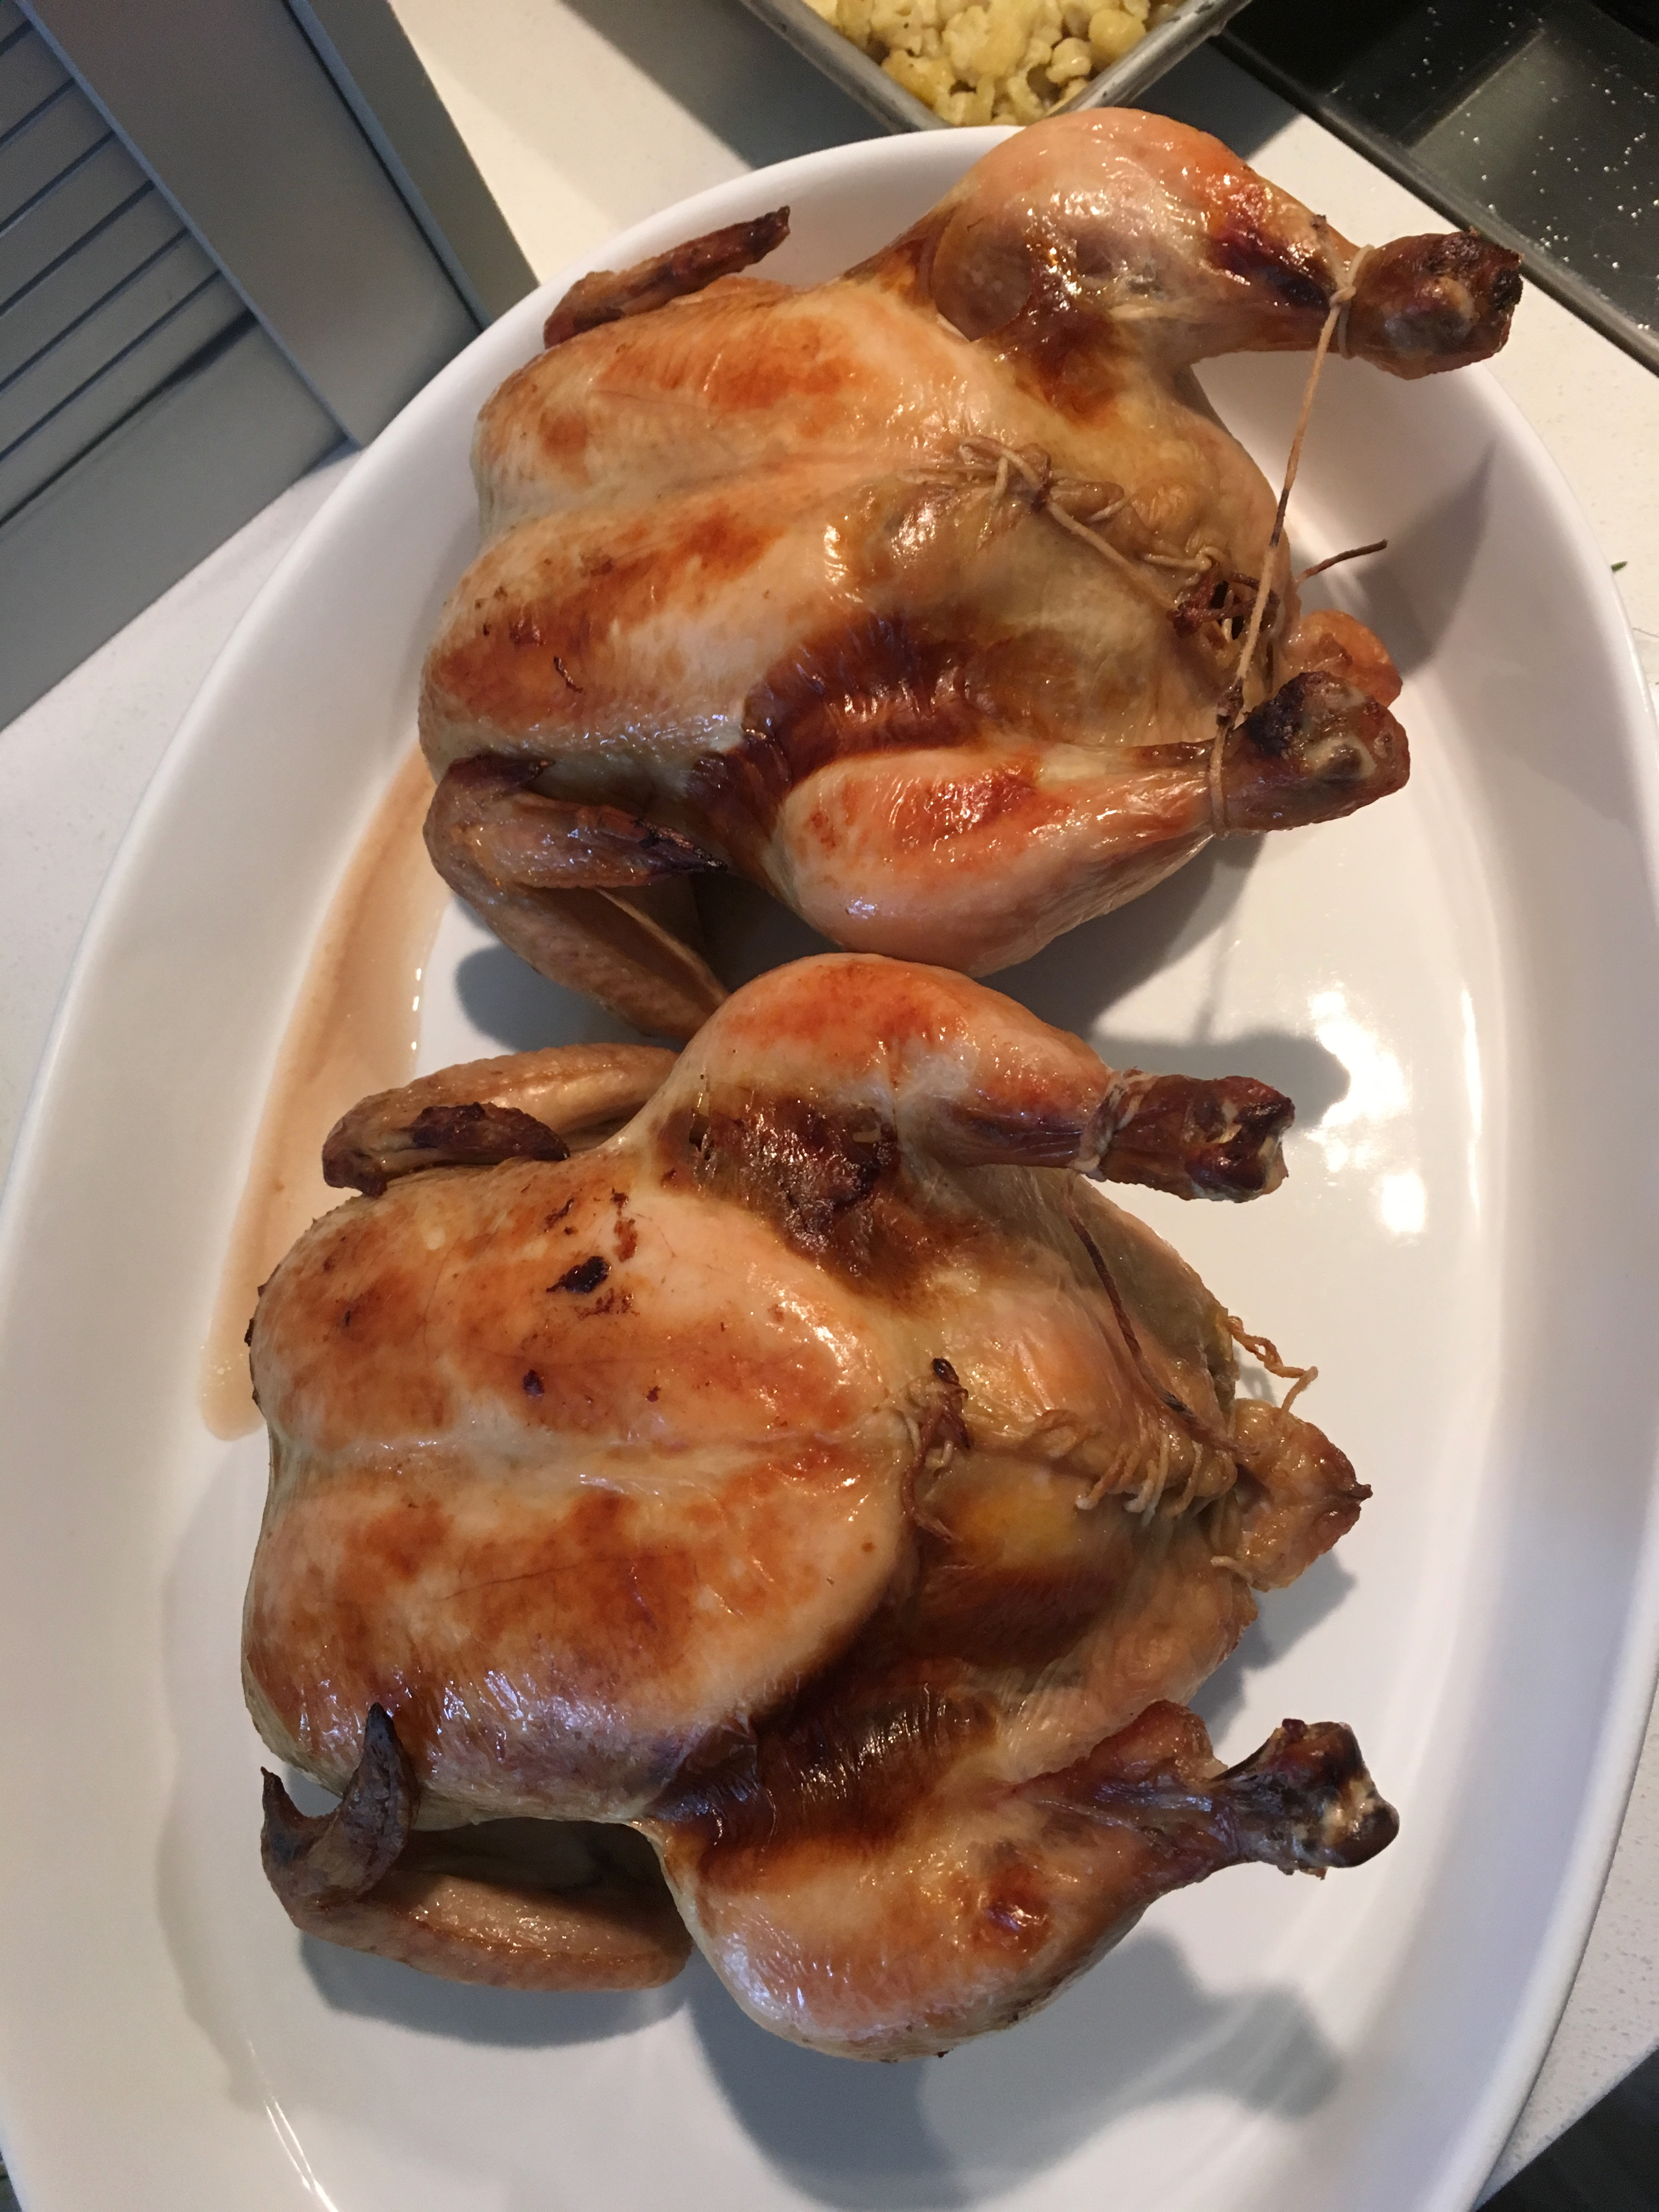
\includegraphics[width=0.25\textwidth]{\imageDir/\fileName/IMG_3228.jpg} \\
\end{tabular}
\end{table}


\end{document}
